Cominciamo a discutere di qualche argomento di elettronica partendo dalla base, quindi partendo dai segnali che fuoriescono da un rivelatore e l'elettronica associata. Parleremo dei possibili segnali che fuoriescono dai rivelatori, che tipo di segnali possono fuoriuscire, come possono essere trattati, quindi che tipo di elettronica si può utilizzare e come possono essere anche trasportati da un modulo elettronico a un altro. 

\section{Rivelatori visuali}

%La prima domanda che ci faremo è se dai rivelatori sono sempre usciti dei segnali elettrici oppure quando è nata la fisica in realtà questo problema non c'era.

\subsection{Emulsioni nucleari}

I primi rivelatori che furono adoperati soprattutto nel campo della fisica nucleare, grazie ai quali furono effettuati diverse scoperte molto importanti, erano dei rivelatori visuali. Infatti i primi rivelatori erano basati sulla visualizzazione di tracce delle particelle in pellicole fotografiche o emulsioni nucleari, le quali potevano essere impressionate, potendo dunque mostrare il passaggio di particelle. Possiamo vedere un esempio nella seguente figura, raffigurante le tracce che si producono a seguito di un'interazione di uranio-238 con un energia di quasi un GeV per nucleone:
\begin{figure}[H]
   \centering
   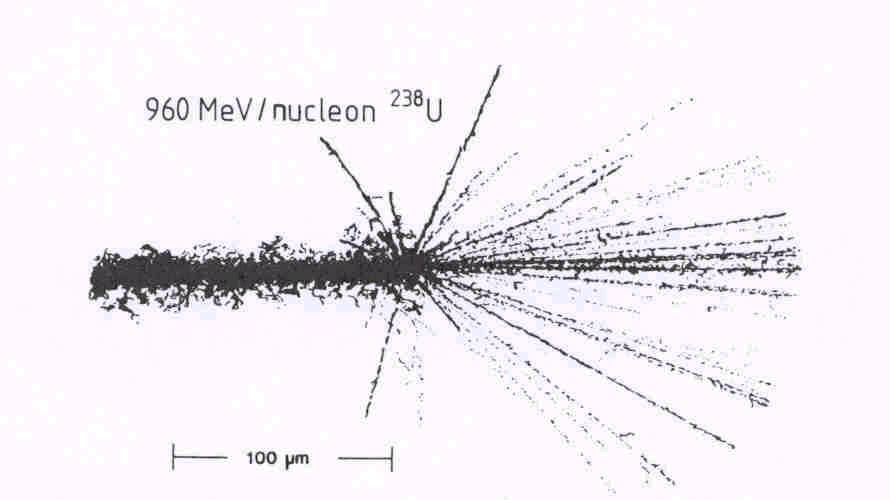
\includegraphics[width=0.6\textwidth]{immagini/emulsione_nucleare.png}
\end{figure}
Questo nucleo di uranio interagisce con un nucleo dell'emulsione nucleare, dando luogo a una serie di prodotti secondari. La traccia più spessa è quindi dovuta al passaggio dello ione pesante, mentre le tracce che vediamo subito dopo sono tutti i prodotti di questa interazione. Tutte queste sono delle tracce lineari.

Oltre all'informazione sul dove è passata la particella, non abbiamo molte altre informazioni aggiuntive, come ad esempio l'energia o il tipo di particella che dà luogo alla traccia. Sebbene quindi abbiamo l'enorme vantaggio di poter visualizzare il percorso di una traiettoria di una particella, al tempo stesso è molto difficile l'interpretazione, cioè avere altre informazioni. Ad essere precisi, abbiamo un'altra informazione: notiamo che c'è un'enorme differenza tra la traccia in ingresso, quella dell'uranio 238, e le tracce prodotte successivamente all'interazione. Il motivo è che lo spessore della traccia dipende dal $\dv*{E}{x}$ della particella, per cui in generale le particelle cariche pesanti, che hanno un $\dv*{E}{x}$ considerevole, in un'emulsione nucleare producono una traccia che ha dimensioni più grandi, tant'è che come vediamo in figura l'$\rm ^{238}U$, che è uno ione pesante, deposita molta energia e di condeguenza la larghezza della traccia è notevole.

Se utilizzassimo un campo magnetico, le particelle cariche comincerebbero a seguire una traiettoria circolare, quindi in quel caso potremmo misurare l'impulso della particella, aumentando le informazioni che abbiamo a disposizione.

Che dimensioni hanno queste tracce? Ovviamente sono tracce molto piccole, dell'ordine di centinaia di micron, dunque devono essere analizzate al microscopio. Questi rivelatori, proprio per le dimensioni che si raggiungono, sono in assoluto i rivelatori che hanno la migliore risoluzione spaziale. Ad oggi però sono dei rivelatori che si utilizzano pochissimo, perché sono dei rivelatori passivi, quindi non hanno bisogno di un'elettronica. Sebbene ciò da ul lato costituisca un vantaggio, dall'altro ci costringe a dover lasciare le emulsioni esposte alla radiazione e quando siamo soddisfatti di quello che abbiamo raccolto le dobbiamo prelevare, sviluppare, quindi trattare chimicamente e poi analizzare in maniera visiva attraverso un microscopio ottico, quindi c'è un tempo morto tra quando avviene l'esposizione e quando avviene l'analisi del dato, pertanto non abbiamo un dato in tempo reale.

Ad oggi sono utilizzate veramente poco, però ci sono degli esperimenti che ancora adoperano le emulsioni nucleari, ad esempio l'esperimento OPERA al Gran Sasso.

\subsection{Camere a nebbia}

\begin{minipage}{0.36\textwidth}
   \begin{figure}[H]
      \centering
      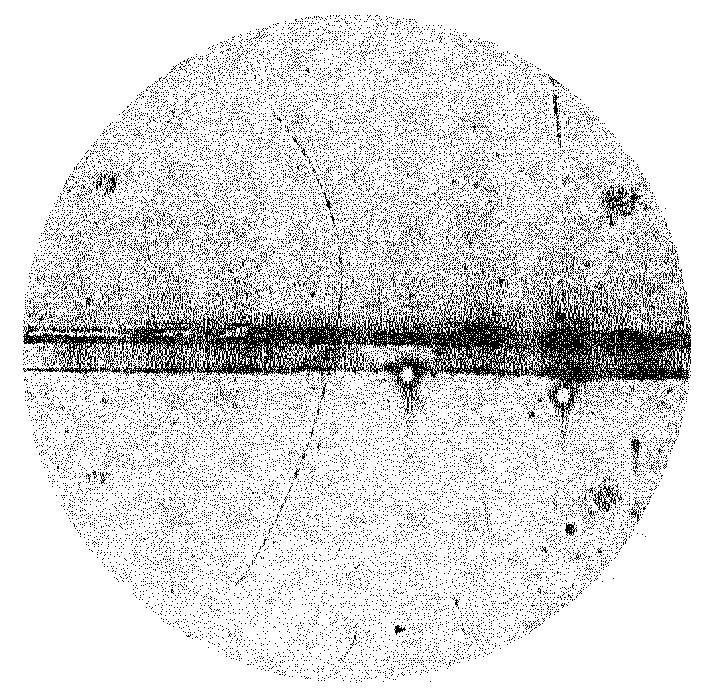
\includegraphics[width=0.7\textwidth]{immagini/camera_a_nebbia.png}
   \end{figure}
\end{minipage}
\begin{minipage}{0.63\textwidth}
   \vspace{0.7cm}Altri esempi di rivelatori che visualizzano le tracce sono le camere a nebbia, che sono dei rivelatori costituiti da camere dove all'interno si crea una condizione di vapore sovra-saturo, quindi una condizione abbastanza instabile, e al passaggio di una particella carica si vengono a creare delle goccioline di condensa lungo la traiettoria della particella.
\end{minipage}

\vspace{0.5cm}Anche in questo caso la dimensione della traccia cambia in base al tipo di particella, ad esempio per particelle cariche leggere vediamo dei percorsi molto sottili a zigzag perché queste interagiscono e cambiano traiettoria, mentre per particelle più pesanti come le $\alpha$ vediamo delle tracce corte e molto larghe.

Anche in questo caso se si accoppia l'apparato con un campo magnetico si può avere qualche informazione in più sulla traccia, però anche stavolta non abbiamo un segnale elettrico ma soltanto una visualizzazione, dunque al massimo possiamo scattare una foto.

\subsection{La camera a bolle}
Un altro esempio di rivelatore visuale è la camera a bolle, che è molto simile alla camera a nebbia però funziona con un liquido e il passaggio di una particella crea delle microbolle lungo il percorso che permettono di visualizzare la traccia.

\begin{figure}[H]
   \centering
   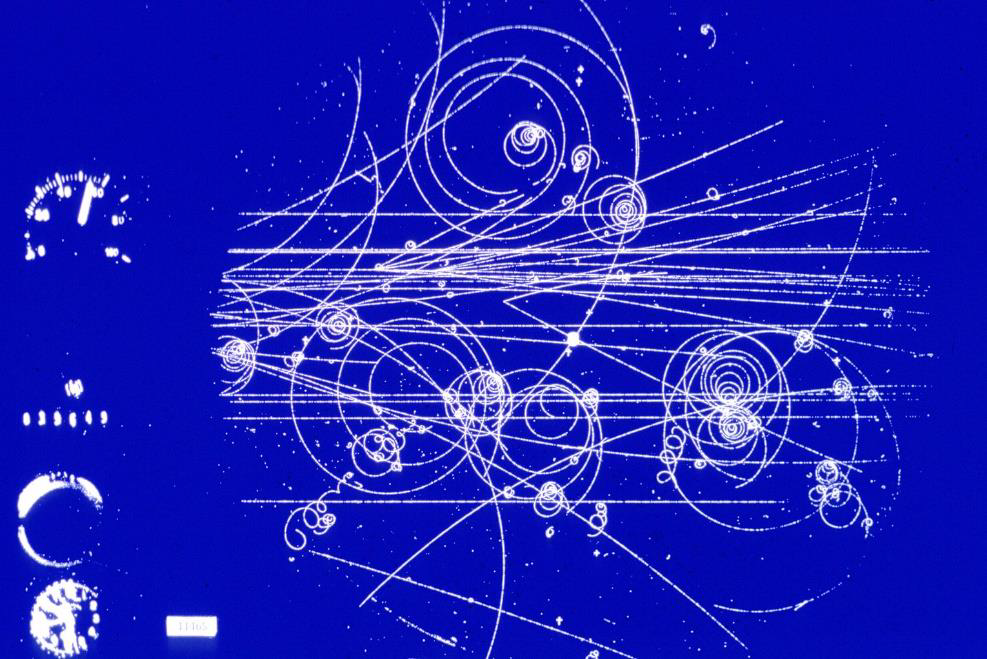
\includegraphics[width=0.6\textwidth]{immagini/camera_a_bolle.png}
\end{figure}

In figura possiamo vedere il percorso che seguirebbe una particella in un campo magnetico, che è una spirale perché man mano la particella perde energia e quindi via via il raggio si riduce.

All'inizio queste tracce si analizzavano a mano. Quello che si faceva era stampare queste fotografie e analizzarle manualmente, che è una procedura molto scomoda.

\section{Rivelatori moderni}

Ad oggi la maggior parte dei rivelatori produce in output un segnale elettrico che può essere di varia natura e che trasporta in sé svariate informazioni, ad esempio sul tipo di particella, sull'energia oppure sul tempo di arrivo.

%\E chiaro che trattare un segnale richiede un'opportuna elettronica. 

Quando parliamo di un segnale, normalmente intendiamo una variazione nel tempo di una tensione o di una corrente.

\begin{figure}[H]
   \centering
   \begin{tikzpicture}
      \draw[->] (0,0) -- (8,0) node[right] {$t$};
      \draw[->] (0,-4) -- (0,1) node[above] {$V$};
      \draw[thick,red] plot[smooth,domain=0:7.7] (\x, {-10*\x * exp(-\x)});
    \end{tikzpicture}
\end{figure}

Generalmente ragioniamo in termini di tensione, quindi su un grafico avente come asse temporale quello orizzontale e come asse delle tensioni quello verticale avere un segnale (impulsivo nel caso della figura) equivale a dire che la tensione dal valore 0 o dal valore di baseline diminuisce o aumenta (a secondo che si tratti di un segnale negativo o positivo) all'improvviso per poi ritornare alla baseline dopo un certo intervallo di tempo. Come abbiamo detto questo segnale può trasportare diverse informazioni, quindi l'elettronica che si adopera a seguire deve essere pensata per estrarre da questo segnale le informazioni che ci servono. Abbiamo già visto un esempio di ciò utilizzando il fotomoltiplicatore in laboratorio: in quel caso sapevamo che l'informazione dal segnale che fuoriusciva dal fotomoltiplicatore che ci interessava era l'ampiezza ossia l'altezza di questo segnale, quindi tutti i moduli elettronici che si utilizzavano a seguire erano finalizzati alla misura dell'ampiezza del segnale, infatti c'era un amplificatore per aumentare l'ampiezza del segnale e un ADC che aveva lo scopo di misurare l'ampiezza e a tradurla in un numero da fornire al computer.

In generale, qualsiasi rivelatore (anche il più semplice) deve prevedere almeno un cavo attraverso cui deve viaggiare non solo la tensione ma anche il segnale che fuoriesce quando viene misurato il passaggio di una particella. Il caso in cui abbiamo un solo cavo è il caso banale, ma in esperimenti complessi, con più canali, bisogna gestire più segnali, dunque servono più cavi\footnote{Per avere un'idea di quanti cavi ci sono e della lunghezza di questi ci basta pensare che in un grosso esperimento a LHC la lunghezza totale dei cavi può essere anche di 3.000 km!}. Ci basta pensare alla camera a fili, in cui da ogni filo esce un segnale.

In ultima analisi, la realizzazione del cablaggio\footnote{Il cablaggio si riferisce all'insieme di fili e cavi utilizzati per collegare vari dispositivi o sistemi elettrici ed elettronici, permettendo il passaggio di energia o segnali.} è un'operazione che può durare anche diverso tempo. A complicare la situazione, si aggiunge il fatto che spesso si cerca di far passare i cavi in appositi passaggi sia per evitare di introdurre del material budget indesiderato nell'esperimento sia perché lo spazio a disposizione non è tutto quello che vogliamo, anche perché in grossi esperimenti spesso si hanno tanti rivelatori diversi a cui lavorano gruppi diversi, per cui è chiaro che bisogna condividere gli spazi. Per tutti questi motivi, il passaggio dei cavi è un'operazione che viene necessariamente studiata dall'inizio di un esperimento.

\subsection{Trapsorto dei segnali}

Cosa viene trasportato in questi cavi?

\begin{itemize}[leftmargin=0.5cm]
   \item Alimentazioni per i rivelatori, i quali normalmente devono essere alimentati o con basse tensioni o anche con alte tensioni, come nel caso del fotomoltiplicatore deve essere alimentato a 600 V, infatti nell'esperienza di laboratorio avevamo il modulo di alimentazione e un cavo che collegava questo fino al fotomoltiplicatore;
   \item Segnali di diversa natura;
   \item Segnali di controllo per le apparecchiature.
\end{itemize}

\section{Segnali impulsivi}
Partiamo innanzitutto andando a vedere che tipo di segnali possono viaggiare in questi cavi.

Come abbiamo detto, per estrarre l'informazione racchiusa in questi segnali è necessario che siano processati con un opportuno sistema elettronico, allo scopo ad esempio di
\begin{itemize}[leftmargin=0.5cm]
   \item distinguere segnali di tipo differente;
   \item estrarre un'informazione sull'energia;
   \item estrarre un'informazione temporale.
\end{itemize}
e ovviamente lo scopo dipende dalla specifica applicazione del rivelatore.

Tipicamente, piuttosto che con segnali periodici, abbiamo a che fare con segnali impulsivi rappresentanti singoli eventi e le informazioni che vogliamo estrarre sono legate alle caratteristiche di questo segnale quali ad esempio l'ampiezza, la durata, la forma del segnale, la polarità, il tempo a cui arriva il segnale e che dipendono dalla misura che stiamo effettuando.

\subsection{Terminologia}
Diamo alcune terminologie importanti quando si parla di segnali. Consideriamo il segnale mostrato in figura, dove è riportato il tempo in ascisse e la tensione in ordinate:

\begin{figure}[H]
   \centering
   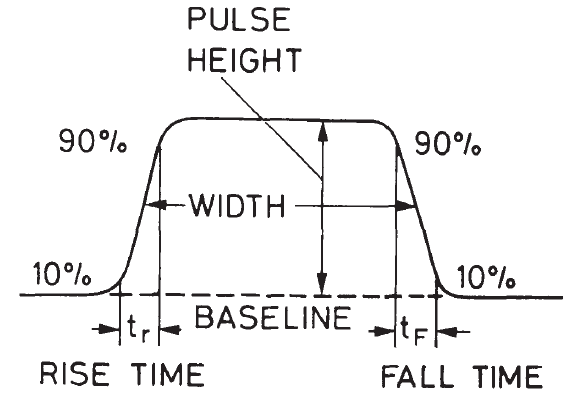
\includegraphics[width=0.5\textwidth]{immagini/terminologia_segnali_1.png}
\end{figure}

Questo segnale parte da un valore costante, aumenta, si stabilizza e poi dopo un po' diminuisce per ritornare al valore iniziale. Si tratta quindi di impulso con una forma un po' più squadrata rispetto a quelle che abbiamo visto in precedenza, ma ci torna utile per dare delle definizioni. Per un segnale, possiamo definire:

\begin{itemize}[leftmargin=0.5cm]
   \item l'\textit{altezza} o \textit{ampiezza} (in inglese pulse height), ossia la distanza tra la baseline e il valore massimo che viene raggiunto dal segnale. In essa potrebbe essere racchiusa ad esempio l'informazione sull'energia depositata nel rivelatore;
   \item la \textit{durata} del segnale, ossia la larghezza (in inglese pulse width),che vediamo rappresentata in orizzontale.
   \item il \textit{tempo di salita} o il \textit{tempo di discesa} (rispettivamente rise time e fall time in inglese), che vengono definiti andando a vedere il tempo necessario perché il segnale passi dal 10\% al 90\% della sua massima ampiezza nel caso del rise time o viceversa dal 90\% al 10\% nel caso del fall time.
\end{itemize}

Il segnale appena visto è un segnale ideale. In realtà si possono presentare dei segnali un po più particolari, con delle deformazioni del segnale, come nella seguente figura:
\begin{figure}[H]
   \centering
   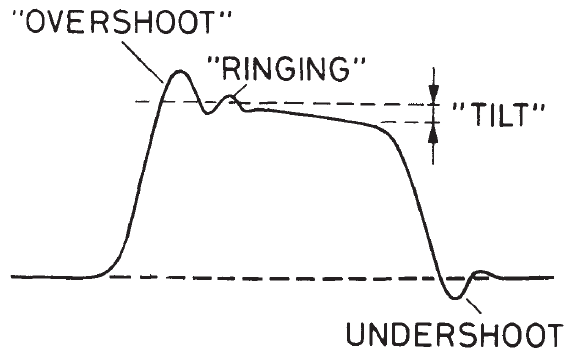
\includegraphics[width=0.5\textwidth]{immagini/terminologia_segnali_2.png}
\end{figure}
Come deformazioni potremmo avere:
\begin{itemize}[leftmargin=0.5cm]
   \item casi in cui il segnale va oltre il valore massimo (detto overshoot);
   \item casi in cui il segnale va al di sotto della baseline (detto undershoot);
   \item effetti di ringing, cioè delle oscillazioni del segnale attorno a un valore;
   \item effetti di tilt, cioè un segnale che dovrebbe essere piatto in realtà man mano presenta una leggera diminuzione della sua ampiezza.
\end{itemize}
Tutti questi sono degli effetti che non vorremmo ma che inevitabilmente, quando il segnale viene trasportato o viene gestito da apparati elettronici, si potrebbero presentare.

\vspace{0.2cm}I segnali potrebbero inoltre essere unipolari o bipolari. Si definiscono unipolari quando presentano un solo lobo, bipolari quando attraversano la baseline.
\begin{figure}[H]
   \centering
   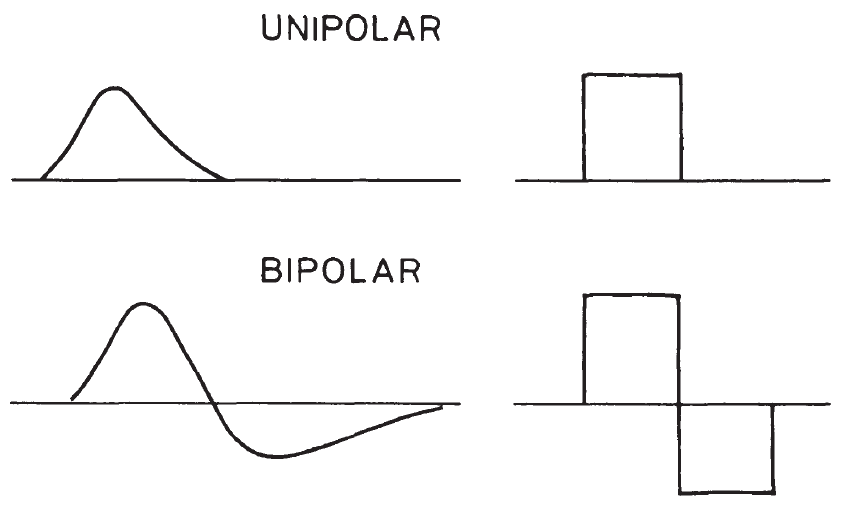
\includegraphics[width=0.6\textwidth]{immagini/segnali_unipolari_e_bipolari.png}
\end{figure}
Nella figura possiamo vedere un esempio di segnale unipolare e uno di segnare bipolare sia nel caso di un segnale analogico che nel caso di un segnale digitale, differenza che spiegheremo a breve.

\vspace{0.2cm}Un'ulteriore distinzione molto importante è quella tra segnali analogici e segnali logici. Nel segnale analogico l'informazione è codificata in modo continuo in una caratteristica del segnale (ad esempio l'ampiezza o la forma) ed è proporzionale al valore dell'informazione. Tornando alla figura precedente, i segnali che vediamo alla sinistra sono esempi di segnali analogici, il cui valore di tensione varia in modo continuo nel tempo. Viceversa, il segnale può essere logico quando può assumere dei valori discreti, dunque la tensione che andiamo a visualizzare all'oscilloscopio non può assumere qualsiasi valore, ma soltanto dei valori discreti. Tipicamente ci sono in totale due valori discreti, perché sono associati allo stato 0 e allo stato 1, e a seconda dello standard ad essi viene associato un certo livello di tensione. \E chiaro che l'informazione che viene trasportata in questo tipo di segnale è inferiore rispetto a quello del segnale analogico, tuttavia essi sono più affidabili poiché è più difficile che l'informazione sia deteriorata nel corso del
trasporto.

Un'altra distinzione che possiamo fare è quella tra segnali lenti e segnali veloci. Questo aspetto si valuta andando a guardare il fronte di salita di un segnale, cioè il tempo che impiega il segnale per passare dal 10\% al 90\% della sua ampiezza. In particolare i segnali si definiscono
\begin{itemize}
   \item veloci quando hanno tempi di salita di alcuni nanosecondi o meno;
   \item lenti quando hanno tempi di salita di centinaia di nanosecondi o anche microsecondi.
\end{itemize}

%Guardiamo adesso qualche tipico esempio di segnale:

\begin{esempio}[Esempio di segnale veloce]
   In figura possiamo vedere la rappresentazione con un oscilloscopio di un tipico segnale veloce:
   \begin{figure}[H]
      \centering
      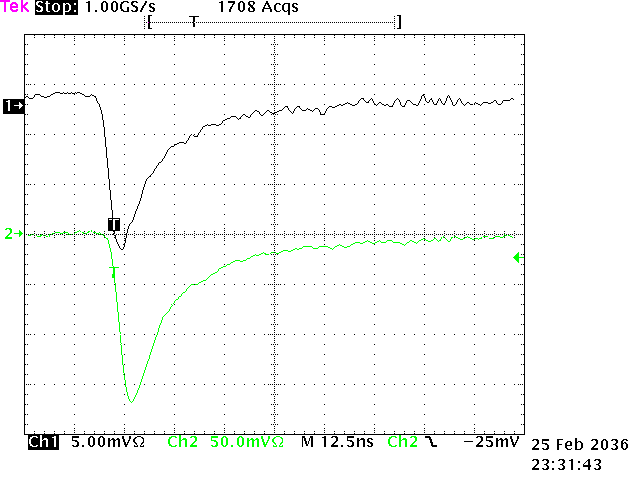
\includegraphics[width=0.6\textwidth]{immagini/esempio_segnale_veloce.png}
   \end{figure}
   Ricordiamo che, in un'oscilloscopio, sull'asse orizzontale si rappresenta il tempo e sull'asse verticale la tensione. Inoltre c'è la possibilità di cambiare sia la scala dei tempi che quella della tensione in base al segnale che vogliamo visualizzare. In questo caso la scala dei tempi (cioè ogni quadrettino) corrisponde a 12.5 ns, mentre la scala verticale corrisponde a 5 mV.
   
   Concentrandoci sul segnale, notiamo che il tempo di salita\footnotemark, cioè il tempo in cui il segnale passa dal 10\% al 90\% del suo valore massimo, ha una durata molto piccola, dell'ordine del nanosecondo, per cui siamo nel caso di segnali veloci.
\end{esempio}

\footnotetext{Anche se il segnale sta scendendo si chiama comunque tempo di salita.}

\begin{esempio}[Esempio di segnale lento]
   Nella seguente figura possiamo invece vedere un tipico esempio di segnale lento:
   \begin{figure}[H]
      \centering
      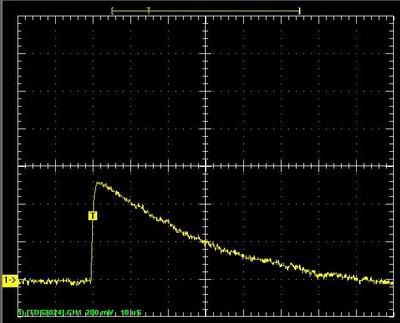
\includegraphics[width=0.6\textwidth]{immagini/esempio_segnale_lento.png}
   \end{figure}
   Notiamo che la scala dei tempi è molto diversa rispetto al caso precedente, infatti stavolta ogni quadretto equivale a $10 \; \rm \mu s$, per cui se ingrandissimo la zona del fronte di salita\footnotemark ci renderemo conto che esso si esaurisce in tempi dell'ordine di centinaia di nanosecondi o anche un microsecondo, quindi siamo nel caso di segnali lenti.
\end{esempio}

\footnotetext{Il fronte di salita è la porzione del segnale in cui avviene la variazione da un livello inferiore a un livello superiore. In pratica, è la fase in cui il segnale inizia a crescere da uno stato basso a uno stato alto.}

I segnali veloci si usano quando siamo interessati all'informazione di timing. Supponiamo ad esempio di voler misurare il tempo di volo di un raggio cosmico nel passare da un rivelatore ad un altro posto alla distanza di 1 metro dal primo: poiché queste particelle viaggiano a velocità prossime a quella della luce nel vuoto, su una base di volo di un metro ci aspettiamo un tempo di volo di $3-4 \; \rm ns$, quindi un segnale lento risulterebe inutile per questa applicazione di timing.

I segnali lenti si utilizzano invece soprattutto in spettroscopia, perché in quel caso non siamo interessati al timing, bensì all'affidabilità sull'informazione legata ad esempio all'ampiezza perché vogliamo misurare l'energia di una particella.

\subsection{Banda passante}
I segnali veloci sono difficili da trattare perché, come vedremo, ogni modulo elettronico presenta una banda passante, e questa ha conseguenze importanti sul segnale che stiamo gestendo.

Per parlare di banda passante dobbiamo immaginare il segnale non più nel dominio del tempo come abbiamo fatto fino ad adesso\footnote{Infatti finora abbiamo studiato i segnali andando a guardare la loro evoluzione nel tempo.}, bensì nel dominio delle frequenze. Per fare ciò utilizziamo la trasformata di Fourier, la quale ci dice che un qualunque segnale (anche aperiodico) rappresentato dalla funzione $f(t)$ può essere decomposto in una sovrapposizione di segnali sinusoidali puri di ampiezza infinitesima:
\begin{equation*}
   f(t)=\frac{1}{\sqrt{2\pi}} \int_{-\infty}^{+\infty} g(\omega) e^{i \omega t} \dd{\omega}
\end{equation*}
dove $g(\omega)$ è la trasformata di Fourier. Invertendo tale relazione si ottiene
\begin{equation*}
   g(\omega)=\frac{1}{\sqrt{2\pi}} \int_{-\infty}^{+\infty} f(t) e^{-i \omega t} \dd{t}
\end{equation*}

Notiamo che l'integrale in $\dd{\omega}$ si estende da $-\infty$ a $+\infty$, il che significa che tutte le frequenze giocano un ruolo nella modellazione della funzione $f(t)$. Pertanto, affinché un dispositivo elettronico possa trattare fedelmente le informazioni contenute in questo segnale, esso deve essere in grado di rispondere uniformemente a un intervallo infinito di frequenze. Ovviamente, in un circuito reale, questo è impossibile. Saranno sempre presenti componenti resistivi e reattivi che filtreranno alcune frequenze più di altre, limitando così la risposta a un intervallo finito di frequenze.

La banda passante di un apparato elettronico rappresenta sostanzialmente l'intervallo di frequenze delimitato dai punti in cui la risposta scende a $-3$ dB. Per comprendere meglio tale concetto facciamo un esempio: immaginiamo di voler adoperare un amplificatore per ascoltare della musica e di averne fissato il guadagno (o come viene detto in gergo di averne fissato il volume) tramite l'opportuna manopola. Idealmente vorremmo che questo amplificatore funzioni allo stesso modo indipendentemente dalla frequenza del suono che stiamo inviando ad esso, ma non è detto che sia così. Infatti potremmo stare lavorando con un amplificatore di scarsa qualità, per cui la risposta cambia in base alla frequenza.

Possiamo vedere un esempio di risposta di un apparato in funzione della frequenza del segnale che stiamo inviando nella seguente figura, dove si rappresenta la frequenza in ascisse e la risposta relativa in ordinate:

\begin{minipage}{0.45\textwidth}
   \begin{figure}[H]
      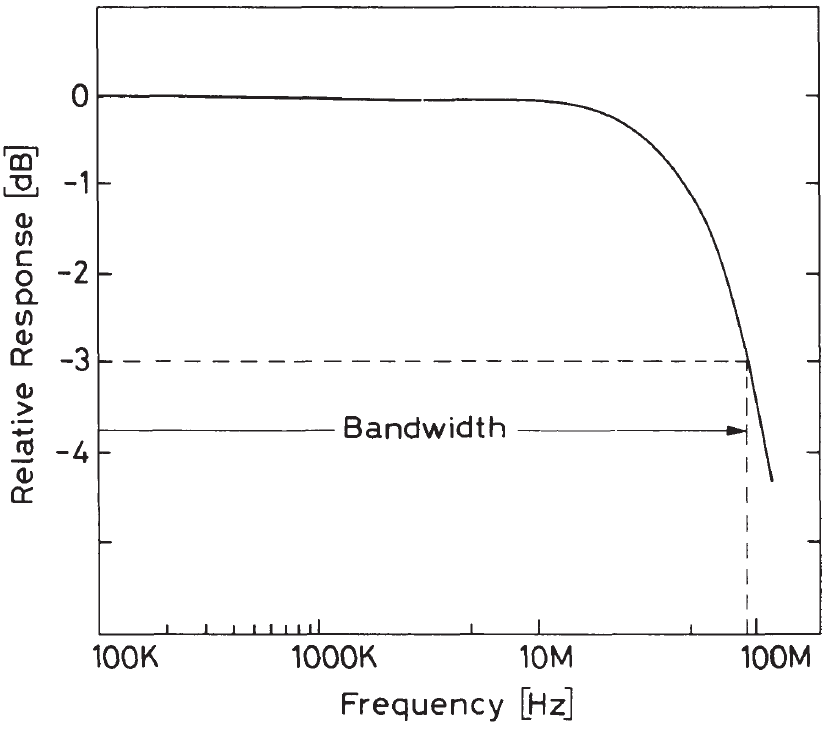
\includegraphics[width=0.99\textwidth]{immagini/banda_passante.png}
   \end{figure}
\end{minipage}
\begin{minipage}{0.54\textwidth}
   Quello che si vede è sostanzialmente una risposta costante, piatta per un certo intervallo di frequenze e poi all'improvviso la risposta dell'apparato elettronico diminuisce. L'intervallo della banda passante è indicato dal punto in cui si raggiunge il limite dei $-3 \; \rm dB$. Se ad esempio riconsideriamo l'esempio dell'amplificatore che utilizziamo per ascoltare la musica, se questo avesse una banda passante a 10 kHz,\footnotemark\, allora tutti i suoni da 10 kHz a 20 kHz non verrebbero riprodotti bene.
\end{minipage}

\footnotetext{Ovviamente non esistono amplificatori per il suono di questo tipo, perché il suono udibile all'orecchio umano arriva almeno a 20 kHz, quindi bisogna certamente superare questa soglia per poter gestire in maniera corretta i suoni.}

Precisiamo che tale limite è imposto per definizione, cioè siamo noi che scegliamo di dire che l'apparato funziona abbastanza bene in tale intervallo di frequenze e che nel momento in cui usciamo fuori da questo intervallo l'apparato non sta rispondendo bene, in quanto c'è un'attenuazione che è più grande di 3 dB.

Vediamo perché si sceglie proprio questa soglia. Ricordiamo che un deciBel è un decimo di Bel ed è definito come segue
\begin{equation*}
   1 \text{ dB}
   =10 \log_{10} \qty( \frac{V_1}{V_2} )
\end{equation*}
dove $V_1$ è la tensione in entrata e $V_2$ quella in uscita.
Vediamo a cosa corrisponde, secondo questa definizione, il valore di 3 dB: sostituendo si ha
\begin{equation*}
   10 \log_{10} \qty( \frac{V_1}{V_2} )=3
   \implies
   \log_{10} \qty( \frac{V_1}{V_2} )=0.3
   \implies
   \frac{V_1}{V_2}=10^{0.3}=1.995 \approx 2
\end{equation*}
Il risultato trovato ci dice che il segnale in uscita si è sostanzialmente dimezzato (cioè è stato attenuato della metà) rispetto a quello in entrata.

In sintesi, definire la banda passante di un modulo elettronico equivale a dare l'indicazione sull'intervallo di frequenze entro cui un apparato di questo tipo funziona correttamente, quindi il segnale viene riprodotto bene. Se ritorniamo alla rappresentazione del segnale mediante trasformata di Fourier, la banda passante rappresenta l'intervallo di integrazione della trasformata. Vediamo allora, nel caso di un segnale impulsivo, come questo venga modificato a seconda dell'ampiezza della banda passante. Osserviamo la seguente figura, in cui è rappresentato un segnale impulsivo di tipo logico a cui di volta in volta è sovrapposta la trasformata di Fourier (indicata dalla linea tratteggiata) ottenuta per diverse ampiezze della banda passante:
\begin{figure}[H]
   \centering
   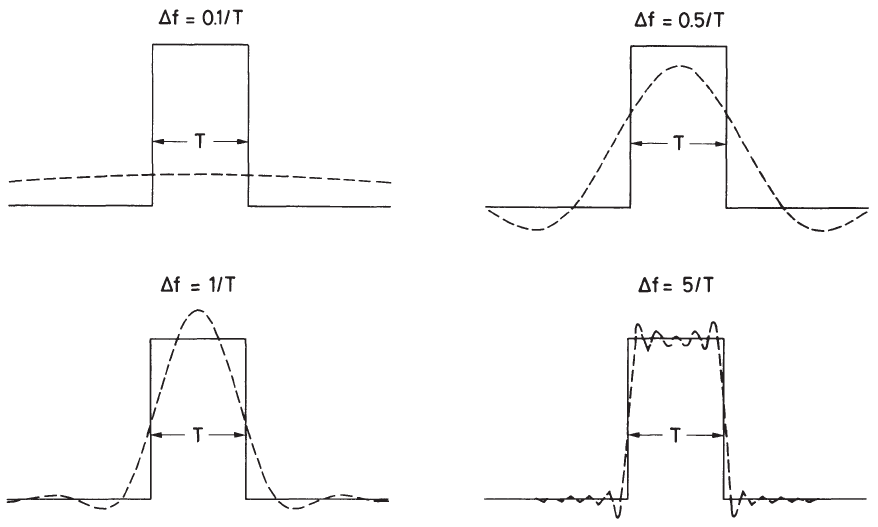
\includegraphics[width=0.8\textwidth]{immagini/banda_passante_segnale_impulsivo.png}
\end{figure}
Detta $T$ la durata del segnale, andiamo a studiare i casi in cui la banda passante ha ampiezza $\Delta f$ pari a multipli di $1/T$:
\begin{itemize}[leftmargin=0.5cm]
   \item Se $\Delta f=0.1/T$, che nel caso in cui $T=1 \; \rm \mu s$ equivale a 100 kHz, il segnale risulta completamente deformato, apparendo quasi piatto;
   \item Se $\Delta f=0.5/T$, che nel caso in cui $T=1 \; \rm \mu s$ equivale a 500 kHz, si vede una sorta di impulso, ma la forma è completamente diversa da quella squadrata che avevamo mandato in ingresso;
   \item Se $\Delta f=1/T$, che nel caso in cui $T=1 \; \rm \mu s$ equivale a 1 MHz, viene riprodotta meglio la baseline rispetto al caso precedente, ma il segnale, di per sé squadrato, viene ancora deformato di molto;
   \item Se arriviamo ad un intervallo $\Delta f=5/T$, che nel caso in cui $T=1 \; \rm \mu s$ equivale a 5 MHz, riusciamo finalmente ad avere una forma più realistica del segnale.
\end{itemize}
Da questo esempio capiamo che l'effetto della banda passante al variare della sua ampiezza è quello di rappresentare il segnale in maniera più o meno realistica, potendo deformare il segnale se scelta in maniera non opportuna. In particolare, possiamo dire che la minima banda passante $\Delta f$ per qualsiasi apparato elettronico per rappresentare in maniera ragionevole l'impulso deve essere almeno superiore a $1/T$, per cui ad esempio per trattare impulsi da 5 ns servono bande passanti di almeno 200 MHz.

Nel caso dell'elettronico nucleare, tipicamente tutti i moduli elettronici hanno bande passanti di almeno 500 MHz. Sebbene non sia banale avere queste bande passanti, ad oggi si sono raggiunti anche limiti più alti, arrivando anche a 1 GHz o 2 GHz in alcuni casi, per cui sono degli apparati ad alta fedeltà, che riproducono in maniera fedele il segnale di ingresso.

\subsection{Da segnali analogici a segnali logici}
Se abbiamo a che fare come un segnale analogico e vogliamo passare a un segnale logico, è necessario utilizzare un modulo elettronico\footnote{Nel seguito vedremo alcuni esempi di moduli elettronici, ma in questo corso non entreremo nel dettaglio del funzionamento di questi moduli, quindi come viene effettuata quell'operazione. Li vedremo come schemi a blocchi, quindi ci interessa sapere, rappresentandoli come dei blocchi, che tipo di segnale entra in ingresso, che tipo di segnale fuoriesce e qual è la funzione di questo modulo elettronico.} che prende il nome di \textit{discriminatore}, il quale ha la funzione di discriminare e dare luogo, partendo da un segnale analogico, ad un segnale logico in uscita. Schematicamente può essere rappresentato nel seguente modo:
\begin{figure}[H]
   \centering
   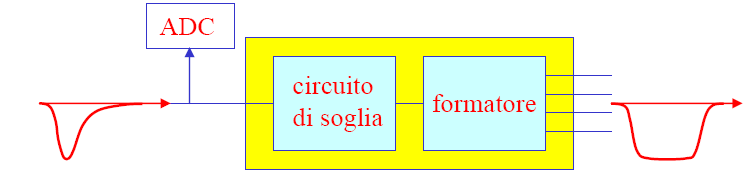
\includegraphics[width=0.8\textwidth]{immagini/discriminatore.png}
\end{figure}
In ingresso abbiamo un tipico segnale analogico, con un valore di tensione che varia in modo continuo nel tempo, e in uscita invece ci ritroviamo un segnale logico che può presentare solamente due valori possibili, o la baseline o un valore massimo.

All'interno un discriminatore deve avere due componenti:
\begin{itemize}[leftmargin=0.5cm]
   \item un circuito di soglia, cioè un circuito che va a confrontare l'ampiezza del segnale in ingresso con una soglia che stabilisce l'utente per decidere se l'altezza del segnale è superiore o no al valore minimo (la soglia) indicato dall'utente;
   \item un formatore, che ha lo scopo di creare in uscita un segnale con un'opportuna forma.
\end{itemize}

Prima di parlare del discriminatore, vediamo gli standard che si usano. Infatti abbiamo detto che un segnale logico è un segnale che varia tra due valori, un valore che rappresenta lo zero logico e uno che rappresenta l'uno logico, ma non abbiamo detto a cosa corrispondano questi in termini di tensione. In altre parole, se mandiamo un segnale logico all'oscilloscopio, che livelli di tensione ci aspettiamo di trovare? La risposta è che dipende dallo standard che si utilizza.
\begin{figure}[H]
   \centering
   \begin{tikzpicture}
      \draw[very thick] (0,0) -- (1.5,0) -- (1.5,2) -- (3,2);
      \node[left=0.2cm] at (0,0) {$0$};
      \node[right=0.2cm] at (3,0) {0 V};
      \node[left=0.2cm] at (0,2) {$1$};
      \node[right=0.2cm] at (3,2) {$2 - 5$ V};
      \node[right=0.2cm] at (3,3) {TTL};
      \begin{scope}[shift={(7cm, 0cm)}]
         \draw[very thick] (0,2) -- (1.5,2) -- (1.5,0) -- (3,0);
         \node[left=0.2cm] at (0,2) {$0$};
         \node[right=0.2cm] at (3,2) {$-0.90$ V};
         \node[right=0.2cm] at (5,2) {0 V};
         \node[left=0.2cm] at (0,0) {$1$};
         \node[right=0.2cm] at (3,0) {$-0.80$ V};
         \node[right=0.2cm] at (5,0) {$-1.75$ V};
         \node[right=0.2cm] at (3,3) {NIM};
         \node[right=0.2cm] at (5,3) {ECL};
      \end{scope}
   \end{tikzpicture}
\end{figure}

Uno standard molto diffuso è il cosiddetto TTL, che è uno standard che prevede che lo zero logico corrisponda a 0 V, mentre l'uno logico corrisponda a un valore che normalmente varia tra i 2 e i 5 V.\footnote{Dal punto di vista ideale dovrebbe essere 5V, ma in realtà c'è una certa tolleranza da parte dei diversi circuiti, tanto che tutto ciò che è al di sopra dei 2 V viene considerato come stato logico uno.} Ad esempio gli ingressi digitali di Arduino lavorano in standard TTL, per cui se vogliamo mandare ad Arduino un segnale logico e vogliamo che sia presente il segnale, dobbiamo mandare un livello superiore ai 2 V. In quel caso, l'ingresso digitale individua l'arrivo di un impulso.

Lo standard TTL non è l'unico. Ad esempio, nel campo della fisica nucleare, spesso si adopera lo standard NIM, dove il livello logico uno corrisponde a una tensione negativa, infatti passiamo da 0 V a $-0.8$ V. Come possiamo vedere dalla figura sopra, la forma del segnale è sempre squadrata ma è al di sotto dello zero, mentre con lo standard precedente è al di sopra.

\comment{

\begin{figure}[H]
   \centering
   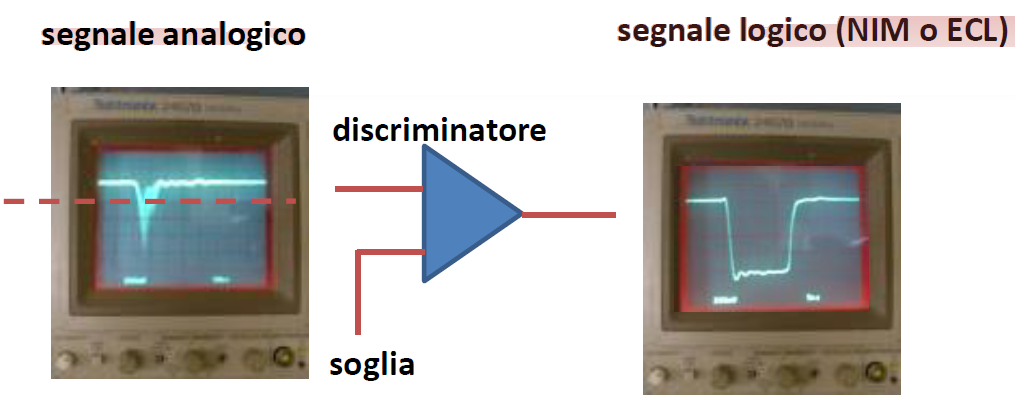
\includegraphics[width=0.8\textwidth]{immagini/segnale_discriminatore.png}
\end{figure}

\textbf{continua a 1:09:50 circa}


Nel caso dei discriminatori, quindi, vi dicevo, abbiamo in ingresso un segnale analogico come quello che, ad esempio, vedete qui visualizzato all'oscilloscopio. Applicate e decidete una soglia al di sotto della quale il segnale viene scartato, non viene presso in considerazione. E attraverso questo circuito di soglia e un formatore, l'uscita si ottiene un segnale logico con un determinato standard. Ora questo è uno specifico, non mi ricordo del cos'è, comunque certamente non è un TTL, perché vedete il segnale è una forma quadrata negativa, quindi sarà quasi certamente un NIM. Quindi questo valore di soglia lo stabilisce l'utente che funziona a un discriminatore, permette ad esempio di andare a scartare, non prendere in considerazione il vostro sistema di acquisizione, eventi in cui l'ampiezza del segnale è al di sotto di un certo valore. Magari avete degli eventi dovuti a del rumore elettronico che tipicamente hanno ampiezze molto piccole, allora io posso utilizzare un circuito di discriminazione per andare a scartare e non considerare tutti i segnali al di sotto di un certo valore, perché magari so che quei segnali non sono di interesse fisico ma sono più legati a un rumore elettronico. Questo, ad esempio, era presente nell'esperienza di gamma, però poi non lo vedevate, sostanzialmente perché era qualcosa che si impostava via software. Benevolato, accorgere solamente perché lo spettro che acquisivate nei primi canali era sempre vuoto. Partiva da un certo canale in poi, se non sbaglio canale 30. Questo perché c'era impostato una soglia al di sotto della quale non veniva misurato nulla, anche quello era sostanzialmente un discriminatore. O beh, questa è una slide che riassume sempre i segnali logici che abbiamo misprima. 

\section{Cavi}
A questo punto, prima di andare a parlare di più nel dettaglio dei diversi moduli elettronici, vediamo come i segnali possono essere trasmessi. Quindi il segnale fu riesce da un rivelatore o deve passare da un modulo elettronico a un altro, come lo faccio, lo faccio attraverso dei cavi. E chiaramente parlo di cavi, non parlo di fili, proprio per indicare il fatto che qualcosa di diverso, non è un semplice filo elettrico, come potrebbe essere, ad esempio, quello che quelli che avete utilizzato in Arduino. In Arduino avevate sostanzialmente dei fili elettrici, non avevano dei propri cavetti, un pin che entrava in un connettore e portava il segnale da un'altra parte. Sembra qualcosa di apparentemente banale trasportare un segnale, ma in realtà non è così, perché l'abbiamo visto, il segnale potrebbe subire delle deformazioni nel trasporto o anche nell'ingresso verso un modulo elettronico, soprattutto se è di natura analogica, quindi un segnale di cui ci interessa conoscere l'ampiezza o altre informazioni. Quindi non bisogna deteriorare chiaramente la qualità delle informazioni contenute nel segnale. Ora, vi dicevo, idealmente noi vorremmo avere bande passanti infinite, ma poi nei fatti siamo dutti, siamo costretti a utilizzare delle bande passanti limitate. Quindi da un lato abbiamo questo problema della banda passante, dall'altro abbiamo la necessità di trasportare dei segnali su distanze che possono essere anche decine di metri e incorriamo ovviamente in problemi concreti. E allora guardiamo la struttura di un classico cavo che viene adoperato per trasportare del segnale. Allora, la struttura è quella che vedete qui rappresentata in figura. Abbiamo sostanzialmente un conduttore interno che è proprio importante del segnale, poi abbiamo un dielettrico di separazione tra segnale e massa, abbiamo una maglia che è uno schermo di fili intrecciati che rappresenta appunto la massa, quindi è un altro materiale conduttivo, poi il tutto viene racchiuso da una guaina di protezione di materiale classico. Quindi ovviamente voi al esterno non vedete nulla se non questa guaina di protezione, ma all'interno dovete immaginare che il cavo è costituito da questa struttura, questo è un tipico cavo coassiale. In realtà ci sono cavi anche più complessi, però quelli che adoperiamo in generale il laboratorio hanno questa caratteristica. La presenza del dielettrico comporta il fatto che il segnale viaggi a una velocità inferiore a c, e quindi il cavo induce un ritardo. Tipicamente per i cavi che adoperiamo si parla di ritardi di 5 nanosecondi ogni metro. E' così importante veramente questa informazione del ritardo che tante volte i cavi vengono classificati non per lunghezza, ma per ritardo. Quindi se vi capiterà poi il laboratorio di far attenzione a questo aspetto, andate a guardare nei cavi l'estremità. L'estremità c'è riportato una piccola spesso, volete riportato una piccola etichetta dove è riportato il ritardo di quel cavo. E tipicamente se prendete un cavo da un metro vi ritrovate appunto stampato 5 nanosecondi. Capite che questo è un modo utile eventualmente proprio per creare appositamente il ritardo. Magari siete interessati ad avere una linea di ritardo, quindi ritardare un segnale rispetto a un altro. Questo se il ritardo è piccolo lo potete effettuare mettendo semplicemente del cavo. Chiaramente da un lato introduce il ritardo, ma dall'altro ricordatevi sempre che il cavo introduce anche un attenuazione, quindi più lungo il cavo più segnale si attenua. Quindi se siete interessati ad esempio al trasporto di un segnale logico e lo volete ritardare, dato che del segnale logico ci interessa poco l'attenuazione, ci interessa soltanto il fatto che ci sia o non ci sia, ma che diminuisca leggermente l'ampiezza non è un problema, allora in quel caso si potrebbe adoperare il cavo, magari decine di metri di cavo per poter produrre un ritardo desiderato. Ci sono tantissime tipologie di di cavo disponibili sul mercato che hanno caratteristiche molto diverse, l'un ed l'altro possono essere coassiali come quello che abbiamo visto prima o anche tri-assiali e comunque quello che si fa è andare a vedere quando si diavesce di un cavo, andare a vedere le caratteristiche, non solo le caratteristiche geometriche in termini di ad esempio in diametro o appunto se di tipo qualsiasi e pericassiale, ma anche altre informazioni come può essere appunto il ritardo, la capricità, l'attenuazione, sono tutte informazioni che servono quando si deve progettare un apparato e un trasporto di segnale. I più utilizzati sono quelli che sono riportati in questa tabella, 

l'RG174 che è la tipologia di cavo che abbiamo adoperato fino adesso ad esempio per l'esperimento dei gammali, quindi un cavo abbastanza sottile vedete un diametro di 0,152 centimetri e ha una esistenza, un'impedenza di 50 ohm, questa è importante, ora lo vedremo per il discorso di adattare il segnale in ingresso ai diversi apparati elettronici. Infatti quando il segnale viaggia in un cavo e entra in un modulo elettronico ci dobbiamo assicurare che le impedenze del cavo e del modulo siano ben adattate, perché quello che potrebbe succedere è una riflessione del segnale, una parziale riflessione del segnale e chiaramente questo è un effetto indesiderato perché potrebbe comportare delle distorsioni del segnale. Allora come faccio a sapere e a valutare l'effetto di questo adattamento dell'impedenza, si può valutare questo coefficiente di riflessione del segnale banalmente appendo a guardare la differenza delle impedenze tra il cavo e il carico esterno, quindi z meno z con 0 e dividerlo per z più z con 0. Allora capite che se le impedenze sono esattamente identiche, quindi immaginate di prendere questo cavo come abbiamo fatto il laboratorio, il cavo che trasportava il segnale del fotomoltiplicatore l'ho mandato all'oscilloscopio, l'oscilloscopio è un carico esterno anche questo, ha una sua impedenza di ingresso, allora se l'impedenza dell'oscilloscopio non corrisponde con quella del cavo che era 50 ohm ho un problema di riflessione quindi io mi devo assicurare che l'oscilloscopio abbia un'impedenza di 50 ohm per poter vedere correttamente il segnale. Infatti se le impedenze sono uguali vedete che questo coefficiente di riflessione è pari a 0 che è quello che vorremmo avere effettivamente. Se invece l'impedenza esterna fosse 0, cioè ci fosse un cortocircuito, rho sarebbe uguale a meno 1, siamo nella condizione estrema, nella condizione opposta estrema, allora in questo caso avremmo una riflessione del segnale e il segnale avrebbe totalmente riflesso, quindi una riflessione uguale ed opposta al segnale. Se invece le impedenze sono uguale abbiamo detto il caso ottimale perché rho è uguale a 0 e non sia alcuna riflessione. Quindi quando vedete ci sono tanti aspetti bisogna tenere in conto quando si deve trasportare a un segnale il tipo di cavo con le sue caratteristiche ma anche l'adattamento al carico esterno. Quindi in generale è necessario terminare quindi collegare un cavo qualsiale con la sua resistenza caratteristica proprio per evitare le distorsioni del segnale. In questa tabella che ovviamente riporto così giusto per esempio ma c'è sono diverse altre nelle slegge successive sono riportate alcune tipologie di cavi, quindi vedete le sigle in alto, ad esempio c'è l'RG174 di cui vi parlavo prima che prende il nome di cavo l'EMO, quindi a volte magari sentirete nominarà anche questo il laboratorio. Vedete queste sono alcune caratteristiche, ne guardiamo alcune, l'impedenza 50 ohm ma non è detto che sia uguale per tutti, ad esempio ci sono dei cavi a 75 ohm, pensate ad esempio al cavo dell'antenna che avete a casa allora tipicamente è un cavo che ha una impedenza di 75 ohm. Quindi ora magari voi state vedendo queste cose qui il laboratorio ma dovete fare anche un lavoro mentale per capire cosa vi può tornare utile anche per quello che vi vede nella vita quotidiana quindi anche il problema di trasportare il cavo, il segnale all'interno del cavo dell'antenna di casa, quanta volta avete avuto problemi con la tv, penso un po' tutti perché è sempre un problema che poi viene risolta anche in maniera molto empirica, dove sta il problema? Sono gli stessi problemi che stiamo affrontando adesso per il trasporto dei segnali quindi la lunezza del cavo come può influenzare il trasporto del segnale, innanzitutto c'è una attenuazione più è lungo il cavo più il segnale 7, dove l'attenuazione, come vedete qui? Espresso in decibel ogni 100 metri quindi mi dice di quanto si attenua il segnale ogni 100 metri ma la cosa importante che vedete da questa tabella è che non è la stessa per tutte le frequenze. L'attenuazione cambia a seconda della frequenza quindi ad esempio volete vedere i segnali della tv e dovete sapere qual è l'attenuazione alle frequenze tipiche dei segnali della tv. Per capire se il cavo che è stato adoperando è un cavo di buona qualità altrimenti appunto bisogna scegliere il cavo più adatto. Come faccio a fare questi conti? Quindi ad esempio qui vedete tabulate l'attenuazione ad alcuni valori di frequenza ma magari voi avete volete sapere qual è l'attenuazione a un esatto valore di frequenza. Come faccio ad avere queste informazioni? Esistono innanzitutto dei CD web che vi permettono di fare questi conti ma esistono i cosiddetti nomogrammi. Un nomogramma è un grafico come quello che vedete qui. Sostanzialmente sono tre grandezze che vengono riportate sulle loro scale ad esempio qui abbiamo riportato la distanza di guardiamo in unità europei in chilometri e l'attenuazione in decibel e in questo caso la frequenza. Allora conoscendo due di queste informazioni potete rinforzare attraverso un nomogramma la terza ad esempio sapete il tipo di segnale che volete trasportare in particolare la frequenza? Immaginiamo 5.000 megahertz quindi il mio segnale a 5.000 megahertz. Lo voglio trasportare a una certa distanza, voglio capire qual è la distanza massima qui lo posso trasportare senza perdere qualità nel segnale e allora conosco l'attenuazione del mio cavo del cavo che voglio adoperare quindi ad esempio in questo caso 142 decimbe all'ogli 100 metri allora unisco questi due valori e vado a vedere l'intercetta nella terza scala allora questo mi dice che io posso trasportare senza problemi un segnale di 5.000 megahertz con un cavo di attenuazione 142 decimbe all'ogli 100 metri fino a una distanza di 50 chilometri oppure viceversa conosco la distanza conosco la frequenza voglio sapere qual è quella attenuazione deve avere il al massimo il mio cavo per poter trasportare in maniera corretto il segnale quindi questi 9 grammi servono proprio per effettuare questi conti o in alternativa si può anche utilizzare si possono utilizzare dei desiti web online che effettuano questi conti quindi sembra un'operazione facile il trasporto dei segnali ma in realtà dietro ci sono tanti tanti aspetti che bisogna tenere in considerazione vi dicevo l'attenuazione si esprime in decimbe all'ogli 100 metri potete anche voi fare il vostro quanticino se ad esempio non vi ritrova le tabulate il valore esatto ad esempio qui abbiamo il valore ogni 50 megahertz magari il vostro quello che vi interessa è compreso fra questi valori non sono 300 megahertz quindi non è riportato il dato come faccio a conoscerlo esiste una una formula che quella che vi è riportata qui dove sostanzialmente dovete conoscere la lunghezza del cavo dovete conoscere il valore di attenuazione ad una data frequenza e da questa formula potete calcolare la perdita totale del cavo a una frequenza che decide voi quindi ci sono ovviamente siti online ma anche delle semplici espressioni che potete adoperare voi stessi facciamo i connettori poi per oggi finiamo ovviamente questo riguarda i cavi ma i cavi all'estremità hanno necessariamente un connettore che tipo di connettori esistono ovviamente anche qui oltre a diversi cavi ci sono anche svariati connettori quindi possono essere connettori pensati in maniera specifica per i segnali come ad esempio i connettori bnc connettori lemo poi li vedremo in laboratorio per i cavi a 50 ommo oppure dei connettori pensati per le altte tensioni come questi svhv mhv e più oltre alla tipologia oltre al tipo di segnale che devono gestire ci sono anche diverse tipologie possono essere connettori maschi femmine connettori atti connettori a e così via ad esempio questo è uno tipico connettore che prende il nome di bnc questo lo avete visto il laboratorio ad esempio i connettori che noi metterò in ingresso allo oscilloscopio magari non l'avete notato però ora che vi faccio vedere la prossima volta che entrerei del laboratorio vi rendete conto un po vedrete dal vivo quello che vi sto dicendo è composto da diverse parti perché vedete a un pin centrale poi a un ground esterno qui vedete l'isolante e non è neanche facile assemblarlo bisogna avere degli attrezzi specifici per per assemblare questo tipo di connettori e comunque sia anche una volta scelto connettore poi ce ne possono essere diverse tipologie qui vedete ad esempio un bnc che viene completato con un atti questo sempre potrebbe servire per suddividere il segnale e quindi crearne una sorta di copia anche se non è una copia esatta perché in realtà il segnale si divide quindi se il segnale in ingresso una certa ampiezza in uscita dalle due t dalle due estremità dell'apt avete un segnale che avrà un'ampiezza che è la metà oppure avete avete bisogno di collegare due due cavi e quindi potreste avere bisogno di una i come quella rappresentata qui quindi semplicemente per creare una connessione insomma c'è veramente una una varietà enorme di di connettori e vi ricordo che tutto ciò che si introduce per trasportare i segnali può creare delle distorsioni un adattamento di impedenza sbagliato abbiamo detto un po comportare una riflessione una parziale di stessione il segnale ma questo anche cosa si traduce si traduce ovviamente in una distorsione del segnale quegli effetti che abbiamo visto prima di overshoot undershoot ring in tilt potrebbe effettivamente presentarsi a seguito di un'elettronica non ottimizzata ma bene ragazzi ci fermiamo qui per oggi ci vediamo giù sono domande sì di me la domanda era se la riflessione si usa al nostro favore no è qualcosa che è assolutamente in desiderato allora qui chiudo la registrazione e la connessione rivederci ragazzi

\textbf{lez. 17}

ok ragazzi allora da fuori mi sentite? si sentiamo ok allora riprendiamo dove abbiamo lasciato la volta scorsa se vi ricordate abbiamo iniziato a parlare di elettronica quindi partendo dai concetti di base in particolare siamo partiti dal discutere i segnali che fuoriescono da un rivelatore quindi abbiamo detto i rivelatori moderni ormai forniscono come uscita un segnale elettronico quindi anzi tutto ci dobbiamo porre il problema di trasportare questo segnale e poi cercare di capire un po la modulistica elettronica che si deve adoperare per poter gestire questi segnali ad avanti questa è un un l'introduzione che abbiamo fatto sui rivelatori se vi ricordate un concetto importante riguardava la banda passante ora lo riprendiamo un attimo vi ricordo che appunto un segnale si può immaginare come una tensione che varia nel tempo quindi come se avessimo un grafico dove sulla stessa orizzontale si riporta il tempo e poi poi poi verticale la tensione in realtà ci possono essere anche segnali in carica segnali in corrente però la cosa più semplice da immaginare soprattutto perché poi è quello che noi visualizziamo uno sceloscopio e un segnale in tensione quindi come quello che vedete rappresentato in questa figura in realtà la forma del segnale può essere anche diverso quello vediamo abbastanza squadrato ma in realtà potrebbe essere un segnale impulsivo molto più stretto quello che ci interessa è capire le principali caratteristiche quindi la larghezza, l'ampiezza, il rise time ognuna di queste può trasportare delle informazioni che possono essere utili ai fini della nostra misura diciamo che in generale per quello che abbiamo fatto fino adesso ci siamo interessati più che altro all'ampiezza del segnale cioè l'informazione che noi volevamo ricavare dal nostro esperimento dalla nostra insura riguardava più che altro una misura di magari energia depositata in uno scintillatore che poi veniva tradotta in ampiezza del segnale un attimo spendo la luce c'è fatto era l'ultima ultima mia e abbiamo anche detto che in realtà il segnale può essere in parte deformato ci possono essere degli effetti indesiderati che modificano la forma del segnale rispetto a una forma ideale e qui vediamo alcuni esempi come un overshoot, un undershoot oppure una diminuzione del segnale, un tilt, un oscillazione o ringing da dove derivano questi effetti lo abbiamo detto possono derivare dall'utilizzo di un'elettronica non adatta a gestire quel tipo di segnale sia per questioni di banda passante sia per questioni magari di problemi di adattamento dell'impedenza perché è importante che il segnale quando viaggia attraversi nella nostra catena elettronica non subisca delle riflessioni abbiamo detto che ogni qualvolta ci ritroviamo una differenza in impedenza tra ad esempio il cavo e il carico il segnale viene in parte riflesso e questo può comportare delle deformazioni indesiderate del segnale quindi bisogna stare attenti a questi aspetti una distinzione importante, lo ricordo, l'abbiamo fatta la volta scorsa è tra analogico e logico a volte anziché parlare di segnale logico si parla di segnale digitale ma in realtà è più corretto dire segnale logico la differenza è che che analogico è un segnale che varia con continuità e assume quindi tutti i valori compresi fra un valore minimo e un un massimo mentre un segnale logico è un segnale che possume solamente due valori di tensione quindi varia tra un livello che noi identificiamo da un punto di vista logico come livello zero cioè non c'è segnale ha un altro livello di tensione che noi identificiamo come livello uno che ci dice che invece c'è segnale e quindi tipicamente è un segnale che ha una forma a gradino capite che l'informazione trasportata da questo segnale è un'informazione binaria c'è o non c'è quindi un'informazione molto più di base rispetto a quella che possiamo avere in un segnale di tipo analogico tuttavia abbiamo il vantaggio che questi sono segnali che difficilmente sono deteriorati nella nostra catena elettronica però chiaramente l'informazione è limitata questi livelli che vi dicevo che corrispondono a gli stati logici zero e uno sono livelli che dipendono dallo standard che è stata doperando ci sono diversi tipi di standard uno standard molto diffuso che avete visto anche in Arduino e lo standard TTL andiamo a cercare di ritrovo segnale TTL dove si varia tra due livelli che abbiamo detto corrispondono a livelli logici zero e uno lo zero corrisponde effettivamente a zero volto l'uno corrisponde a un valore compreso fra i due e cinque volt nominalmente dovrebbero essere cinque volt però anche se sia un valore un po' più basso normalmente l'elettronica lo riconosce comunque sia come un segnale presente vi dicevo questo è uno standard che avete sperimentato dal vivo perché alla fine Arduino, sostanzialmente la parte digitale di Arduino tratta segnali di questo tipo quindi segnali si dice positivi perché il livello uno è un livello che si trova a un potenziale positivo rispetto al livello zero ovviamente squadrati quindi una forma quadrata la durata quella poi dipende ovviamente dalla particolare applicazione altri standard prevedono diversi livelli in particolare il laboratorio spesso ci ritroveremo con questo standard NIM dove questa volta abbiamo un segnale negativo cioè il livello zero corrisponde sempre a zero volt mentre il livello uno corrisponde a meno 800 mili volt quindi richiamato un po' questi questi di base sul segnale riprendiamo la banda passante per ricordare l'importanza della banda passante di un apparato elettronico questa banda passante se vi ricordate è la risposta tipica di un sistema in funzione della frequenza e ci dice che all'interno di questo intervallo di frequenze il nostro sistema fornisce una risposta che è all'isopra di meno 3 decibel è più chiaro forse con una rappresentazione grafica come quella che vedete qui dove si riporta la risposta relativa di questo apparato dove zero sostanzialmente corrisponde a una risposta ideale e vedete come al variare della frequenza è arrivata a un certo punto la risposta del sistema si attenua e quando si arriva alla soglia di 3 decibel a quel punto siamo al limite della banda passante la banda passante di uno strumento è importante perché ci permette di trattare i segnali nel modo più fedele possibile avevamo fatto proprio l'esempio di questo segnale impulsivo un segnale impulsivo di forma quadrata quindi questo segnale l'abbiamo visto logico indipendentemente dall'ampiezza non ci interessa in questo momento ci siamo più che altro concentrati sulla durata per capire come in base alla banda passante il segnale viene rappresentato e viene trattato quindi se segnali si può immaginare da un punto di vista matematico come espresso attraverso questo integrale dove G è la trasformata di Fourier un integrale tra meno infinito e più infinito ci domandiamo se anziché fare questo integrale nell'intervallo da meno infinito e più infinito ci fermiamo nell'intervallo della banda passante cos'esce fuori per F quindi se F è questa in partenza andando a limitare l'intervallo di frequenza a un valore pari a 0.1 diviso T dove T è la durata del segnale ci rendiamo conto che il segnale viene parecchio deformato e quello rappresentato nella linea tratteggiata questa situazione migliora a mano mano mano mano chiaramente la banda di frequenza diventa più ampia vedete che con un intervallo pari a 5 su T abbiamo una rappresentazione molto più fedele del segnale chiaramente più è alta la banda passante più il segnale viene riprodotto freddelmente non mi ricordo esattamente dove eravamo arrivati magari mi aiutate voi a ricordarlo questo l'hanno fatto sì, sì l'hanno fatto anche i sunnerd avevano fatto anche tutta la parte dei cavi dell'impedenza vero? ok ok questo l'hanno finito? no no, non eravamo arrivati qua ok, va bene questo era un grafico per ricordare le distorsioni che fosse avere i segnali in base ovviamente a problemi di impedenza allora completiamo questa parte sui segnali abbiamo parlato della produzione dei segnali, del trasporto e adesso parliamo della visualizzazione qualcosina l'abbiamo già viste in laboratori insieme, penso con un po' tutti tutti gruppi il modo più semplice per visualizzare un segnale che viaggia attraverso un cavo e quello di inviarlo a uno sciloscopio lo sciloscopio lo possiamo banalmente immaginare come se fosse un voltmetro quindi uno strumento che misura una tensione una differenza di potenziale e che lo rappresenta in un grafico in funzione del tempo quindi banalmente nel monitor dello sciloscopio quello che si visualizza è sull'asse orizzontale, l'asse temporale, sull'asse verticale invece un'asse in tensione, in volt in realtà questa ovviamente è una rappresentazione molto banale dello sciloscopio oggi gli sciloscopi vi dicevo sono degli strumenti molto sottisicati che sono anche in grado di effettuare diverse operazioni anche delle vere misure online, quindi quello che avete fatto voi utilizzando un ADC esterno e un PC a volte può essere già trovato, lo potete trovare già all'interno dello sciloscopio integrato e quindi alla fine viene prodotto un spettro delle ampiezze e dei segnali che hanno andato allo sciloscopio quindi ci sono sciloscopi ovviamente molto performanti la più grande distinzione, la principale distinzione è tra sciloscopi analogici e sciloscopi digitali probabilmente negli l'abburatori degli anni passati avete avuto a che che con sciloscopi analogici quindi col monitor ricoperto, florescente mentre quello che avete visto in l'abburatorio è un esempio di sciloscopio digitale questo è lo schema di base di uno sciloscopio analogico, cosa vediamo innanzitutto potremmo avere più ingressi quindi mi permette di visualizzare simultaneamente più segnali ovviamente la scala temporale sarà comune entrammi segnali, la scala verticale mi ricordo se in quello analogico si può fare mi sembra di sì, si può ottimizzare per ogni segnale la cosa più importante da ricordare sullo schema di funzionamento di uno sciloscopio analogico è il fatto che questa traccia che viene visualizzata su questo monitor viene prodotta attraverso un fascetto di elettroni che viene fatto debiare utilizzando delle placchette orizzontali e placchette verticali a cui si applicano delle differenze di potenziale opportune allora sulle placchette orizzontali che determinano il movimento del fascetto orizzontalmente si applica una tensione a venti di sega quindi una tensione che fa sì che questo fascetto sostanzialmente viaggi lungo l'asse orizzontale poi improvvisamente torni indietro e lo fa ciclicamente sull'asse verticale, quindi sulle placchette verticali si va ad applicare la differenza di potenziale che corrisponde al segnale da visualizzare quindi questo fascetto chiaramente verrà debiato in base al valore di tensione che gli sta arrivando in ingresso e quindi il risultato alla fine è una traccia visibile che a volte anche abbastanza 

permanente sul monitor dello sciloscopio anche lo sciloscopio ha una sua banda passante e anche in questo caso dobbiamo capire l'effetto che potrebbe avere nella visualizzazione del segnale in particolare ha effetto, ha importanza quando si va a valutare il tempo di salita di un segnale quindi immaginate di inviare un segnale anche abbastanza veloce con un tempo di salita che quindi chiamo con T-Rice ora in realtà quello che visualizzarete all'o sciloscopio sarà un tempo indicato qui con T-Mage che è dato dalla somma in quadratura del tempo effettivo di salita del segnale più un tempo dettato dalle caratteristiche dello sciloscopio quindi questo che modifica un po' lo sciloscopio allora questo tempo caratteristico dello sciloscopio si valuta conoscendo la banda passante che è indicato con questa F-310 belle e utilizzando questa formula che è una formula approssimata quindi conoscendo la banda passante dello sciloscopio e Sperse \& Medias potete valutare a quanto ammonte eventualmente questo contributo dovuto allo sciloscopio quindi un segnale che magari ha un tempo di salita di due mano secondi in realtà poi allo sciloscopio lo vedrete leggermente più lento dovuto a questo contributo che però se lo sciloscopio di buona qualità diventa, lo capite bene voi stessi diventa un contributo abbastanza trascurabile perché appunto più grande la banda passante più questo valore è veramente piccolo e trascurabile l'impedenza in ingresso è in generale alta proprio perché è caratteristica di uno strumento come un voltmetro ma in realtà quando è inviato un segnale con un cavetto LEMO di cui abbiamo parlato la volta scorsa che è una impedenza a 50 ohm conviene adattare le impedenze del cavo e del carico in questo caso e quindi all'interno dello sciloscopio è possibile possibile modificare l'impedenza lo stadio di ingresso può essere in diverse modalità, può può in continua che la modalità normale di funzionamento oppure può essere in AC cioè viene filtrata la componente in continua oppure in ground cioè l'ingresso è posizionato al ground in generale possiamo avere anche dai due ai quattro ingressi indipendenti questo più o meno è quello che appare normalmente su un display di uno sciloscopio l'avete visto in presenza voi stessi quindi abbiamo diverse manopole che possiamo modificare per agire ad esempio sulla scala verticale e quindi cambiare quella che la scala quindi quanti mili volte corrisponde ogni divisione potete anche spostare il segnale quindi mettere uno shift in verticale oppure la stessa cosa la potete fare in orizzontale quindi variare la scala in orizzontale per cercare di vedere maggiori dettagli del segnale e potete anche aggiungere un ritardo e quindi spostare orizzontalmente il segnale rispetto alla scala abbiamo anche parlato se vi ricordate quando vi ho fatto vedere lo sciloscopio del trigger il trigger è un concetto di base della fisica in generale per trigger si intende una condizione che fa partire l'acquisizione di un evento o in questo caso nel caso dello sciloscopio la visualizzazione del segnale io potrei essere interessata a vedere soltanto alcuni segnali che hanno un certo significato un certo valore e altri non non visualizzarli perché magari non mi interessano o viceversa quando avete a che fare con un sistema di acquisizione che acquisisce preliminary preliminary è una una una fa fa fa fa fa fa fa fa fa fa fa fa fa fa fa fa fa lo vedremo tra qualche slide si parla di un sistema di trigger ad esempio la cosa più semplice che potreste fare, guardando un po' quello che avete fatto il laboratorio e nell'esperienza in cui avete misurato l'energia dei gamma gamma e e è messa da sorgente potete decidere di mette una condizione potete decidere di mette una condizione e per per trigger e una condizione di questa imponente e quindi quando è verificata e verificata viene viene del dato chiaramente quando parliamo di oscilloscopio non parliamo di ver di ver di di di perché non acquisiamo dati intermedibight per visualizzazione visualizzazione e per un oscilloscopio il trigger può essere in anzitutto o interno o esterno interno se fa riferimento al segnale stesso che voi inviate e quindi ponete una condizione sul segnale oppure può essere esterno cioè acquisisco quando viene inviato quando ricevo un segnale esterno ok quindi sono di la voldue cose indipendenti l'input è il segnale di trigger questi sono belli questo è come appare uno oscilloscopio analogico che penso che avete visto in altre occasioni quindi con tutte le manopole che abbiamo visto schematizzate in quella figura qui ci sono i diversi ingressi e il monitor che vi permette di visualizzare i segnali lo oscilloscopio digitale appare molto più carino anche molto più compatto tutti i venti quello sembra un reperto storico però le funzionalità sono analo che quindi lo scopo e lo stesso possiamo provare a fare un confronto cioè che differenza c'è tra quello analogico e digitale al di là del funzionamento in sé in termini di prestazioni voglio capire ma è meglio uno oscilloscopio analogico oppure uno oscilloscopio digitale diciamo ci sono prove e contro ne abbiamo parlato anche in laboratorio in generale ecco vi devo dire di quello digitale come differenza rispetto a quello analogico ha il fatto che il segnale viene acquisito quindi all'interno c'è un ADC che va a campionare il segnale in un certo numero di punti e lo rappresenta poi nel grafico come se fosse un segnale per punti chiaramente tanto più fedele tanto più e tanto più fedele quanto più è grande il numero di punti che utilizza per rappresentare una forma donna quindi quella che noi chiamiamo frequenza di campionamento capite se di una forma donna intera prende tre punti ovviamente la rappresentata è male più punti ci sono quindi più è fitto il campionamento più il segnale viene rappresentato in modo fedele quindi capito tutto viene a questo punto digitalizzato e allora se li confrontiamo possiamo in anzi tutto fare delle considerazioni sulla curatezza quindi quanto bene il segnale viene riprodotto e allora nel caso dell'oscilloscopio analogico questo dipende esclusivamente dalla banda passante lo abbiamo detto prima nel caso dello oscilloscopio digitale questo dipende dalla banda passante ma anche dalla frequenza di campionamento ok quindi solo due effetti che si vanno a sommare ovviamente poi abbiamo una differenza per quello che riguarda la sovrapposizione delle forme donna normalmente nell'oscilloscopio lo utilizziamo per acquisire un solo segnale per volta l'abbiamo visto anche in laboratorio, arriviamo a un segnale poi dopo un po' di tempo ne arrivava un altro però non vedevamo forme donna sovrapposte ma potreste invece essere interessati a vedere delle forme donna sovrapposte per capire nel tempo se l'ampiezza magari ci sono delle ampiezze preferite più frequenti e quindi se immaginate tanti segnali che si sovrappongono l'un all'altro ci saranno delle zone più denze dovevo dire appunto che quel segnale con quella ampiezza si è presentato con maggiore frequenza ora questa modalità è presente in entrambi i oscilloscopi sia quello analogico che quello digitale in quello analogico si sfrutta sostanzialmente la permanenza della traccia nello schermo quindi la memoria del fosforo in quello digitale invece è ovviamente un'operazione software che dipende anche dalla capacità dell'oscilloscopio di memorizzare più forme donne e poterle rappresentare simultaneamente nello schermo quindi all'inizio effettivamente gli oscilloscopi digitali primissimi modelli non riuscivano a riproburre bene questo effetto, questa modalità ma adesso effettivamente sono competitivi tanto quanto quelli analogici poi un'altra cosa che possiamo ecco che fa una differenza importante riguarda il trigger quindi quando acquisire questi eventi quando vederli e allora nel caso di quello analogico ovviamente il trigger si può fare solamente sull'ampiezza del segnale quindi dico voglio vedere soltanto segnali più grandi più ampi di 8 millivolt questa è l'unica condizione che posso imporre in quello digitale invece normalmente è possibile adoperare trigger più complessi che magari possono derivare anche da combinazioni logiche di segnali quindi immaginate ad esempio di avere un oscilloscopio digitale con 4 ingressi e di mandare a ciascun ingresso dei segnali in input sono interessati magari soltanto a vedere la forma donda quando la coincidenza tra tutti e 4 ecco questo si può fare da un punto di vista software utilizzando un oscilloscopio digitale per quello analogico non si potrebbe fare dovremmo fare noi la coincidenza in partenza produrre un segnale di coincidenze cioè dire ora parleremo anche della coincidenza comunque penso che è arrivata a intuire il concetto di coincidenza cioè quando due segnali arrivano allo stesso istante simultaneamente nel caso di quello analogico sono costretta a realizzare una coincidenza a parte con una modo listica dedicata produrre un segnale di trigger che deve essere inviata al segnale all'uscizoscopio analogico per eventualmente acquisire i segnali quindi un po' più complesso e inoltre quello digitale vi dicevo proprio per il fatto che digitalizza l'informazione la trasforma in byte in dati che noi possiamo salvare ci permette proprio di fare delle operazioni quindi non solo lavorare sul trigger ma anche di fare degli analisi e dei segnali in tempo in tempo reale vi dicevo si possono produrre già degli spettri per i modelli più avanzati quindi in generale ci sono delle funzionalità che quello analogico non possiede ci sono domande completo questa parte con questa idea che visto che abbiamo fatto appunto questi kit da utilizzare a casa con materiale abbastanza economico quindi il kit sul multimetro e il kit che utilizzano Arduino in realtà anche per quanto riguarda l'utilizzo di un uscizoscopio si può fare qualcosa a livello casalingue nel senso con costi molto bassi infatti sono stati immessi nel mercato degli uscizoscopi piccolini ovviamente magari a un solo canale che però hanno dei costi abbastanza contenuti dell'ordine di qualche decina di euro, venti, trenta euro e che permette di visualizzare segnali magari non segnali veloci come sono quelli che escono ad esempio da rivelatori come scintillatori o altro però segnali lenti come quelli che ad esempio avete gestito con i sensori di Arduino ecco se volete visualizzare qualcuno di questi segnali è possibile comprare uno di questi uscizoscopi tassalinghi che si presentano ad esempio come questo, questo viene dato in commercio, bisogna montare il pannello alla parte dell'elettronica però diciamo l'assemblage è molto semplice e vedete che prevede un solo ingresso con un connettore BNC che è uno dei connettori che abbiamo discusto la volta scorsa poi abbiamo un cavo con due puntali quindi questi puntali si adoperano proprio per andare a prelevare il segnale in alcuni punti ad esempio se avete a disposizione un sensore come quelli che avete operato per Arduino un'altra che alimenta il sensore potete provare a prelevare il segnale e visualizzarla all'uscilloscopio vedete sono dimensioni molto compatte decine di centimetri, il display è abbastanza piccolino però diciamo prevede la possibilità 

di fare un po' tutte le operazioni che si fanno tipicamente con oscilloscopio, qui sono riportate ad esempio le caratteristiche, possiamo vedere che la scala verticale varia da 10 mili volte 5 volte quindi è ottima la scala orizzontale è un po' più più vedete non potete andare al di sotto dei 10 microsecondi quindi non potete vedere segnali veloci se vi ricordate in laboratorio per visualizzare i segnali che venivano prodotti dallo scintillatore del fotonottibilitatore era necessario spandere la scala e renderla 20 nanosecondi per divisione, 10 non secondi per divisione quindi non siamo a questi livelli però per segnali lenti va più che bene tutte le modalità di trigger, auto, normal, singolo insomma tutto quello che fa un oscilloscopio professional ovviamente in scalari d'otta la larghezza della banda non è eccezionale ma d'altra parte ci lo aspettavamo, segnali veloci non li possiamo gestire perché la banda passante non ciò permette questo è un altro modello un po' più compatto ma anche più o meno meno stesso costo, monta addirittura il processo del primo, vedete qui lo schermo come è come appare, come permette di visualizzare i segnali più super rendervi i parteci di del fatto che esistono anche questi prodotti in commercio che sono veramente galini, veramente simpatici ci sono domande? allora proseguiamo andando a discutere i principali moduli che potremmo doverare in elettronica quindi noi faremo riferimento a moduli che utilizzeremo durante il laboratorio ma anche a moduli che sono presenti in tantissime attrezzature scientifice quindi independentemente dal fatto che uno puoi fare il fisico nucleare l'astrofisico, lo strutturista comunque sia ci sono dei moduli di elettronica che sono alla base di un sistema di trattazione dei segnali e quindi vedremo quelli più comuni più utilizzati in anzitutto questo è lo standard NIM potremmo anche saltarlo allora quello che noi vedremo in laboratorio riguarda l'utilizzo di moduli che rientrano in questo standard che chiamiamo standard NIM non confondiamolo con quello del del segnale per vostere scusi non mi posso otterne hai ragione si si ok doverse vederlo adesso comunque sono questo è uno standard che nasce nel campo della fisica nucleare allora al di là del fatto che voi utilizzerete questi moduli nello specifico vi dicevo in realtà la funzionalità di alcuni moduli elettronici è importante conoscerla al di là proprio dello standard poi adoperato quindi che cosa consiste nello specifico questo standard consiste nell'adoperare in anzitutto dei segnali che hanno tutte queste caratteristiche quindi questi moduli che possono essere amplificatori, discriminatori unità di coincidenza allora a mano andremo a vedere sono tutti i moduli che si aspettano di gestire segnali in questo standard NIM quindi sempre 3-0 e 800-800 mili volte perché questa caratteristica perché un tempo molto tempo fa i tempi di fermi quando si progettava un esperimento in realtà era il fisico stesso a produrre la propria elettronica quindi in base a quello che si doveva fare si produceva l'elettronica ad hoc ma a mano che si è andata avanti nel tempo ci si rese conto che era importante anche per lavorare meglio in collaborazione con altri gruppi era importante creare uno standard quindi cercare di rendere quanto possibile standardizzati questi moduli quindi un primo passo è stato fatto utilizzando questo standard NIM che trattava gestiva dei segnali che avevano tutte le stesse caratteristiche e questo rese è tutto più facile perché è anche con l'avvento dell'elettronica commerciale quindi sono nata delle ditte che hanno proprio prodotto questi moduli elettronici allora a quel punto era necessario introdure uno standard, cosa che prima non era previsto questo standard NIM ormai è un standard abbastanza vecchio nato nel 1964 però fa la sua funzione già avevo accennato questi moduli non prevedono un'alimentazione stand alone cioè un'alimentazione con una presa da attaccare alla presa di corrente al muro ma in realtà vengono banalmente alimentati utilizzando questo contenitore che avete visto anche in laboratorio che prende il nome di Crate e appunto un contenitore dove si fanno a inserire in questo slot diversi moduli quindi può alimentare diversi moduli di tipologia NIM in questo caso in parallelo infatti qui sul retro vedete questi connettori che servono semplicemente a fornire delle tensioni standard delle tensioni che sono presenti in queste unità sono queste la più o meno 6 la più o meno meno la più o meno meno quindi tutti i moduli previsti in questo standard utilizzano tutte o parte di queste tensioni quindi alcune magari non le prendono in considerazione altre invece le vengono utilizzate quindi per adoperare in qualsiasi modulo basta inserirlo in questo slot accendere il Crate quindi l'alimentazione viene fornita in questo modo questi Crate però sono caratterizzati dal fatto di non avere intelligenza a bordo quindi non ci sono processori a bordo e semplicemente un Crate che assicura l'alimentazione di questi moduli sono utilizzati principalmente nei sistemi di trigger veloci quando si vuole produrre un un segnale di trigger in modo pronto in modo veloce e allora che tipo di moduli possiamo adoperare vi dicevo noi non andremo nel dettaglio del modulo specifico lo vedremo attraverso degli schemi a blocchi ci interserà soltanto capire cosa va in ingresso e cosa esce fuori da un modulo quindi qual è la funzione di questo modulo e allora partiamo con quello più semplice una linea di ritardo potrebbe nascere infatti l'esigenza di voler ritardare un segnale quindi il segnale ricordo se ne abbiamo un esempio sì qua, il segnale ovviamente se questa è una setemporale ha un suo inizio un suo start un punto da cui lui in cominci a discostarsi dalla baseline. Questo start potremmo volerlo spostati in avanti, quindi ritardato. Come si fa questa operazione? La cosa più banale che si può fare è ad operare un cavo. Il cavo, se vi ricordate, introduce un ritardo naturale, perché il segnale viaggia a una velocità che è inferiore alla velocità della luce di vuoto, e in particolare abbiamo un ritardo di 5 in media, di 5 nanosecondi ogni metro di cavo. Quindi delle linee di ritardo che noi definiamo passive, cioè dove non c'è nulla di attivo, sono costituite proprio da cavi arrotolati che introducono un ritardo fisso. Quindi queste linee di ritardo passive prevedono anche diversi switch per cambiare la lunghezza del cavo da introdurre e si possono aggiungere ritardi dell'ordine di qualche nanosecondo, 5, 10, 20 nanosecondi, però capite che arrivato a un certo punto c'è un limiter, c'è potete arrotolare tanto cavo, ma poi non potete arrivare ovviamente a ritardi di micro-secondi, perché ci vorrebbero cavi eccessivamente lunghi. In quel caso si deve ricorrere a unità di coincidenza di tipo attivo. In quel caso c'è un circuito attivo che effettua un'operazione di ritardo per ovviamente aggiungere ritardi consistenti di micro-secondi o anche millisecondi. Quelli che vedrete in laboratorio saranno delle linee di ritardo passive. Magari me lo ricordate, vi faccio vedere anche all'interno come sono fatte perché si può smontare il pannello laterale e vedere che all'interno alla fine non ci sono altro che cavi. Oppure un'altra operazione molto comune che si fa in elettronica è quella di realizzare fan-in e fan-out. Il fan-in consiste sostanzialmente in un or logico. Quindi se questo è il modulo di fan-in, in ingresso abbiamo due segnali, immaginate due segnali logici, quindi due deradini, in uscita esce un unico segnale, ogni qualcoltè è presente almeno un ingresso. Quindi per questo si realizza l'OR perché dal punto di vista logico nella tabella di verità dell'OR se vi ricordate, basta che uno dei due segnali in questo caso sia uno, l'uscita sarà uno. Quindi basta che da uno di questi ingressi ci sia un segnale e allora in uscita verrà prodotto un segnale. Questo è uguale esattamente a un or. Il fan-out invece, diciamo, è l'operazione opposta, nel senso da un segnale ne voglio creare una copia. Ora questo si potrebbe fare banalmente utilizzando un connettore a t. Se vi ricordate un connettore a t ve l'ho fatto vedere la volta scorsa, prevede un ingresso, è proprio la forma di una t. Quindi la base dell'attì è l'ingresso. E le altre sono le uscite. Questo permette effettivamente di suddividere il segnale e quindi realizzare una sorta di copia, però qual è lo svantaggio? In questo caso il segnale in uscita risulterà la metà di mezzato in ampiazza. Quindi non è una copia esatta in realtà. Un fan-out verrà proprio, realizza proprio una copia. Quindi se il ingresso ho un segnale in uscita, ho due segnali identici al primo. E questi moduli possono esistere sia in versione lineare che logica. Quindi possono funzionare sia se i segnali sono di tipo logico sia se sono di tipo analogico. Quindi vedete, non stiamo parlando di come funziona all'interno un fan-in o un fan-out, ma la funzione che svolge, quindi che tipo di segnali abbiamo l'ingresso in uscita e che cosa fa il modulo. Quindi riassumendo un fan-in equivale a un or, un fan-out equivale a fare una copia del segnale. Ad esempio, un fan-out ricordato, avrelo passato alla copia, lo possiamo riamare quando parleremo dei discriminatori, perché quando è necessario fare una copia, ora lo vedremo. Un'altra operazione che si fa spesso sui segnali elettrici riguarda la discriminazione. Quindi stabilire se un segnale supera un certo valore di soglia. Questo è utile perché in elettronica bisogna sempre stabilire ciò che può essere un segnale di rumore, dovuta al rumore dell'elettronica, da ciò che invece è un segnale di rilievo. E quindi quello che spesso si fa è guardare il segnale, ad esempio un segnale che ha questa forma, scegliere una soglia e dire se il segnale è più alto di questa soglia, per me va bene. A qui siamo, o visualizziamo l'alloscilloscopio, nuovamente è una sorta di concetto di trigger che abbiamo visto in precedenza. Quindi la discriminazione consiste proprio nel dire se il segnale soddisfa questa condizione, cioè se è superiore a una certa soglia. Sembra una operazione banale, perché alla fine cosa dobbiamo fare? Dobbiamo soltanto confrontare l'ampiezza del segnale con un livello che viene scelto dall'utente. Capite se il livello è troppo basso, si rischia di acquisire segnali molto piccoli che magari sono dovuti al rumore elettronico, se si mette una soglia troppo alta, si rischia invece di perdere segnali anche di interesse dal punto di vista fisico. Ora questo modulo, il discriminatore, in ingresso accetta un segnale analogico, perché su un segnale logico capite che questa operazione non ha molto senso, visto che il segnale logico è sempre la stessa ampiezza, quindi non ha molto senso, cioè lo potete fare, però scoprirete che se vi mantenete con una soglia al di sotto del livello 1, vedrete sempre segnale, altrimenti se vi spostate sopra il livello 1 state discriminando e tagliato ogni segnale. Questo modulo quindi in ingresso vi dicevo accetta un segnale analogico, come quello che vedete qui, e in uscita produce un segnale logico, come quello che vedete qua sotto. Questo segnale dovrebbe partire esattamente quando il segnale in ingresso supera la soglia. 


Quindi vedete se questo è il segnale e questa tratteggiata è la soglia, a questo istante di tempo, lo vedete qua sotto, parte il segnale logico in uscita. La larghezza, la durata di questo segnale logico non dipende da quando il segnale ripassa la soglia, ma viene sabbrita dall'utente. Ok, quindi la durata del segnale logico in uscita è scelta dall'operatore. Ricordato però perché spesso si fa questa confusione, non so perché tanti studenti dicono poi la durata dipende da quando il segnale riempire attraversa la soglia, ma non è così. Quindi quello che conte soltanto il primo punto dove il segnale va al di sopra della soglia, quello è il punto in cui parte il segnale logico, poi la durata viene scelta da chi utilizza il discriminatore. Un'altra cosa spesso viene detta in maniera errone agli esami, io ve lo dico perché poi magari riascoltando le lezioni ci fate più attenzione, il discriminatore non fa passare, spesso dicono il discriminatore fa passare una parte del segnale, no non è così, il discriminatore riceve un ingresso in segnale e ne produce in uscita un altro. Quindi l'unico legame tra segnale in ingresso e segnale in uscita è legato al tempo di partenza del segnale logico, basta. Poi del segnale in ingresso non ci manteniamo nulla, nessuna altra informazione. Ok, ci interessa soltanto quando questo ha attraversato la soglia. Vi dicevo la discriminazione può essere utile per diversi scopi, può essere utile per generare un trigger, quindi stabilire quando visualizzare un segnale, acquisirlo, oppure per misure di tempo, per ad esempio andare a misurare la differenza in tempo tra due segnali, quindi come faccio a sapere quanto tempo intercorso tra due segnali analogici, basta che li discrimino, ne produco due logici, vado a vedere la distanza temporale tra questi due logici. Le soglie si possono regolare chiaramente, lo dicevo, possiamo sceglierla più bassa, più alta, chiaramente bisogna sempre stare attenti, e le larghezze del segnale in uscita vi dicevo sono regolabili, possono essere molto strette, anche pochi nanosecondi, o molto lunghe, anche dell'ordine di microsecondi. Come si realizza questo discriminatore? Quello di cui abbiamo parlato fino adesso è il cosiddetto leading edge, cioè guardando il fronte di salito del segnale si va a vedere quando questo supera una certa soglia, questo algoritmo si imprende il nome di leading edge, ed è ovviamente la modalità più semplice di discriminazione, quindi il modo più semplice per effettuare una discriminazione del segnale, ma in realtà questo ha in sé una problematica, cioè genera una indeterminazione nell'istante di tempo in cui si genera il segnale logico, si crea un jitter, vi faccio vedere direttamente l'esempio. Immaginiamo che questa sia l'asse temporale, che è questo orizzontale, perché questi siano due segnali, ovviamente sono schematizzati, stilizzati, un segnale di ampiazza più piccola e un segnale di ampiazza più grande, che arrivano allo stessistante, quindi idealmente se arrivano alle stessistante, mi aspetto che il segnale del discriminatore parta allo stessistante, ma in realtà non è così perché vedete se questa è blu e la soglia, il segnale di ampiazza più grande intercetterà la soglia all'istante t1, mentre il segnale di ampiazza più piccola all'istante t2, quindi se io immagino che in uscita il segnale logico parta a t1 per il primo segnale e a t2 per il secondo segnale, vedete che c'è una indeterminazione sull'istante a cui viene fatto partire il segnale in uscita, indeterminazione che deriva dal fatto che i segnali possano avere forma diversa, come faccio a eliminare questa dipendenza dalla forma del segnale, si adopera, in questo caso, un discriminatore a un attimino più elaborato, che prende il nome di Cosson Fraction Discriminator, discriminatore a frazione costante. In questo caso il discriminatore scatta, non scatta a una data soglia, ma a una determinata percentuale dell'ampiazza, quindi ad esempio rispetto all'ampiazza massima, ma io voglio che il discriminatore scatti al 50\% dell'ampiazza massima. Quindi non è un livello fissato, 20mV, no, è un livello che cambia secondo dell'ampiazza massima, se mi arriva un segnale di 1V, se imposto come percentuale il 50\%, vuol dire una soglia di 500mV, se arrivasse un segnale invece di 2V, la soglia del 50\% corrisponde a una soglia di 1V, perché questo cambia la situazione, quindi rispetto al grafico di prima, guardiamo ora a Cosson Fraction, che differenza apporta. Quindi per il segnale più piccolo che ha questa ampiazza, vedete che la soglia dovrebbe essere questa, quella più in alto, se ad esempio ci manteniamo al 50\%. Per il segnale più grande in cui l'ampiazza è questa, il 50\% corrisponde a questa soglia di 1V, e vedete che i due segnali attraversano la soglia allo stesso istante. Quindi questo risolve quel problema che è caratteristico degli engaging. Ma allora gli engaging non sono utili? No, sono utili, comunque sia, perché vi dicevo un discriminatore può avere diverse funzioni, ad esempio potrei essere interessato banalmente a togliere segnali di bassa ampiazza. E allora in quel caso il leading edge va benissimo, perché comunque sia basta che vi imposto la soglia a un valore ameguato, faccio quello che per cui ho pensato di utilizzare il discriminatore. Se invece sono interessata ad applicazioni di timing, quindi utilizzare i segnali del discriminatore per fare misure di tempo, allora è chiaro che il leading edge non mi va più bene, deve adoperare un costo on fraction discriminator.


Quindi il discriminatore a frazione costante è più complesso e viene utilizzato soprattutto quando è importante avere un'informazione temporale precisa. Ma come può funzionare un discriminatore a frazione costante? Se ci pensate è un po strano perché qui io sto dicendo devo impostare la soglia a una percentuale dell'ampiazza massima, ma io come faccio a sapere l'ampiazza massima? Ok, è un po' cosa di strano. Ora questo si risolve nel seguente modo con questo piccolo circuitino. Allora il primo passo è suddividere il segnale, farne una copia e qui quindi vi ritiamo il fan out che vi dicevo prima, quindi questo poterizza banalmente un fan out che crea due copie e lo stesso segnale. Una copia viene in anzitutto invertita, quindi vedete cambia polarità. La copia in alto invece viene semplicemente ritardata quindi il risultato è avere un segnale con polarità positiva ritardato rispetto al segnale con polarità negativa. A questo punto si vanno a sommare questi due segnali insieme, questa è la somma, vedete i due segnali in basso uno in alto e questa è la somma. La somma che si ottiene è un segnale bipolar con due lobby uno negative e uno positivo, è un passaggio dallo zero. Quello che si sceglie per come istante per generare il segnale in uscita è proprio il passaggio dallo zero che è indipendente dall'ampiezza del segnale, dalla forma del segnale. Quindi questo è un circuitino molto semplice che utilizza il discriminatore e che ci permette di avere un riferimento temporale che è indipendente dall'ampiezza del segnale. Se volete potete provare anche voi stessi a creare un discriminatore via software, provate a simulare un segnale anche semplicemente per punti, provate a realizzare queste due operazioni, quindi create due copie, una ritardate quindi spostate i punti sull'asorizzontale e l'altra semplicemente la ribaltate, li sommate insieme e doverste ottenere questo risultato. Potreste provare a modificare l'ampiezza del segnale e vedere che questo punto in zero crossing non cambia a seconda dell'ampiezza del segnale. Dove che entri in gioco la percentuale è essenzialmente in questo ritardo, quindi cambiare per cambiare la percentuale di soglia se agisceakesse sul ritardo. Ci stanno domande? Questa? Una scala di conteggio ho detto anche scalar. Ecco, scusate, vi dico un'ultima cosa sul discriminatore. Il discriminatore lo potete fare anche via software, potete anche provare a farlo con Arduino. Banalmente, con Arduino potete acquisire un segnale di insensore e di insensore analogico e decidere di acquisire solamente se quello che acquisite è adisopra di un certo valore, è un semplice liding edge. Quindi, sono operazioni che si possono fare o per via elettronica, se si vuole, gestire il segnale, oppure via software. La scala di conteggio scaler sono semplicemente dei contatori di impulsi logici non digitali, scusate, non modifico, perché sono, poi mi rimane, che mi dico. Ci possono essere anche qui diversi standard, in particolare il laboratorio, troviamo sempre lo standard NIM, quindi sarà sempre un modulo che va inserito in quel crate e presente un piccolo display. Per favore, lo schermo. Ok, ogni volta che scusa la presentazione, no, no, no, no, è che ogni volta che scusa sotto, se non condivido le slide in modalità presentazione. Comunque, ditemelo, si è bloccata, se ci perdiamo il monitor. Allora, vi dicevo, normalmente ci sono dei display dove, a mano, avvengono rappresentati i conteggi, quindi si inviano degli impulsi logici e questo modulo semplicemente conta quanti ne sono arrivate. Banalmente, con un contatore è come quello che avete adoperato durante l'esperienza con il contatore Geiger e l'asorgente Beta. Forse non tutti, perché alcuni hanno adoperato poi il computer perché ci sono stati problemi, però l'apparato di partenza prevedeva una pericchiatura che, oltre ad alimentare il contatore Geiger, aveva un display. Ecco, al suo interno, sostanzialmente, c'è un contatore, gli arriva l'impulso del contatore Geiger e questo contatore conta quanti impulsi arrivano e gli rappresenta su un display. È chiaro che possono lavorare fino a certe frequenze, poi, quando i segnali diventano troppo frequenti, il tempo morto potrebbe essere eccessivo, quindi potremmo perdere informazione. Anche qui potreste realizzarlo con Arduino, quindi, se ad esempio avete in ingresso un sensore di tipo digitale, in quel caso, potete contare quanti impulsi gli arrivano e potete ora presentarlo sul computer, oppure potreste provare a governare uno di questi piccoli display che si collegano per Arduino e, man mano, far vedere l'incremento dei conteggi che arrivano. Le coincidenze. Il concetto di coincidenze l'abbiamo già accennato poco fa, perché comunque è un concetto che utilizziamo anche quotidianamente, non necessariamente riferiti ai segnali elettrici. In che cosa consiste una coincidenza? La coincidenza consiste nell'andare a individuare una condizione per cui due segnali arrivano simultaneamente, allo stesso istante. Ora, capite che dire allo stesso istante non è proprio facile, c'è bisogno di in realtà definire una finestra entro cui due segnali si possono considerare incoincidenza. E quindi questa finestra prende il nome di finestra di coincidenza, si esprime in secondi, perché è ovviamente un tempo, e se due segnali si verificano entro questo intervallo di tempo, allora si definiscono incoincidenza. Ad esempio, qui vedete quello che si può realizzare, una coincidenza che si può realizzare con semplici rivelatori. Qui abbiamo due scintillatori, ognuno colledato al proprio fotomolstibilicatore che è alimentato, vedete con un modulo di alta tensione, dal fotomolstibilicatore che segnale fu riesce, che tipo di segnale fu riesce. È un segnale logico o analogico? Non vi sento quelle mascherine? No. Analogico. Analogico, perché? Perché è un segnale la cui ampiazza è proporzionale all'energia che è stata depositata nello scintillatore. Quindi dall'ampiazza del segnale voglio capire effettivamente quanta energia è stata depositata nello scintillatore. Quindi mi aspetto un segnale, se torno indietro, di questa forma. Ho al massimo invertito, negativo, insomma non ha importanza, gli interessa è semplicemente il fatto che in vari in modo continuo nel tempo. Quindi dovete immaginare che qui su questo cavo sta fagiando un segnale analogico. Allora per realizzare una coincidenza le coincidenze si realizzano soltanto su segnali logici. Quindi prima di arrivare al modulo di coincidenza devo in qualche modo produrre dal segnale analogico un segnale logico. Allora come posso farlo? Utilizzando, vedete, dei discriminatori che sono quelli che abbiamo discusso prima. Quindi il discriminatore riceve l'ingresso, il segnale analogico e produce un segnale logico in uscita. In base alla condizionazione che gli imposto io posso decidere, basta che sopra una certa soglia. Ok? A quel punto questi due segnali logici provenienti dai due rivelatori possono essere ritardati in maniera opportuna e mandati al modulo di coincidenza il quale fa uscire un segnale in uscita solo se i due segnali mi ingresso risultano essere coincidenti entro la finestra temporale. E allora potrei contare con un counter, uno skader, una scala di conteggi che abbiamo visto prima quante coincidenze si sono verificate. Ad esempio perché si potrebbe verificare una coincidenza tra questi due scintillatori perché magari questi sono messi uno sull'altro, arriva un raggio cosmico dall'alto attraverso prima uno e poi l'altro. Quindi mi aspetto che con una differenza di tempo piccolissima i segnali prodotti da questi due suono moltiplicatori siano abbastanza vicini in tempo l'un all'altro che ritardo mi posso aspettare. Un minimo di ritardo me lo posso aspettare perché se ad esempio questi due scintillatori si trovano a un metro di distanza insomma li dovete dare il tempo a questo raggio cosmico di passare da quello in alto a quello in masso. Quindi mi lo aspetto un minimo di ritardo che posso tenere in conto qui giocando su questi due ritardi perché se un segnale ad esempio questo è il primo segnale questo è il secondo segnale. Il secondo segnale è sempre un po' dopo il primo.

Allora potrei riallinearli mettendo un ritardo sul primo segnale perché i due segnali sono fisicamente in coincidenza ma semplicemente per il fatto che c'è di mezzo o un metro di distanza risultano essere lontani in tempo di qualche anno secondo ma questo lo recupero banalmente quando un ritardo, introducendo un ritardo su uno dei due segnali. Quindi in base anche alla fisica devo capire come mettere in tempo questi due segnali. Non so se è chiaro questo aspetto. Un aspetto importante quando si realizza una coincidenza è cercare di capire se la coincidenza è dettata da un fenomeno fisico come può essere effettivamente un cosmico che attraversa i due scintillatori oppure da una casualità. Facciamo un paragone che non c'entra niente con la fisica. E' un'altra persona andiate spesso in un bar 3-4 volte al giorno. Allora non abbiamo tutto questo tempo di disposizione ma immaginiamo questa situazione. Che ci andate casualmente nell'arco della giornata quindi non ora rifissati. Qual è la probabilità che voi e quest'altro amico vi incontriate al bar per caso? Chiaramente una probabilità non nulla può avvenire e quando è bene capite che è stata una casualità, una coincidenza casuale perché non vi siete messi d'accordo per incontrarvi al bar quell'ora ma semplicemente per il fatto che ognuno di voi va all'ispeso e magari sta lì per un certo intervallo di tempo c'è una probabilità non nulla per cui alla fine possiate incontrarvi per caso. Ecco qualcosa di simile la dobbiamo immaginare anche per le coincidenze in fisica. Nel senso ci sono delle coincidenze che hanno origine fisiche quindi se un cosmico attraversa uno scintillatore poi l'altro quella è una coincidenza fisica però potrebbe anche capitare che per caso i due scintillatori abbiano dato un segnale in coincidenza anche se in realtà non è una coincidenza fisica. È chiaro che nel momento in cui io sul contatore vedo un incremento quindi arrivato a una coincidenza io non posso sapere se la coincidenza era una coincidenza casuale o spuria oppure una coincidenza vera però posso stimare o un modo di stimare il livello di coincidenze spuria quindi capire quante me ne posso aspettare quindi se ad esempio io nel contatore poi misuro in un'ora 100 coincidenze posso sapere di queste 100 quante grosso modo sono dovute alla coincidenza spuria, la coincidenza casuale. Ora se ritorniamo all'esempio del bar capite che avere una coincidenza casuale dipende innanzitutto da quante volte voi andate al bar se ci andate quattro volte, se ci andate cento volte in un giorno e da quanto tempo state al bar? Allo stesso modo le coincidenze spuria in questo caso dipenderanno da quante la frequenza di conteggio di ciascuna scintillatore in questo caso, stiamo facendo con l'esempio degli scintillatori ma quei vale dovete immaginare due rivelatori che generano un segnale quindi da la frequenza di conteggio di ciascuno dei rivelatori che equivale a quante volte andate vai al bar e dalla finestra di coincidenza quindi questo intervallo entro cui io considero due segnali in coincidenza e qui vale a quanto tempo voi state al bar. Ora queste due informazioni, ora ci torno un attimo su questa, vi permettono di calcolare la frequenza dei quanti teggi spuri attraverso questa semplice formula due per s0 per s1 per delta t, s0 s1 sono le frequenze di conteggio dei singoli rivelatori quindi si esprimono in hertz, delta t è la famosa finestra temporale che noi stiamo considerando. È giusto per avere un esempio, un'idea, se ad esempio entrambi questi due rivelatori contano 3.000 particelle al secondo con una finestra di 50 nanosecondi che è una finestra anche abbastanza stretta, se vi fate il conto applicando quella formula si trova un rate di coincidenze casuali dell'ordine dell'hertz quindi se poi io nella mia misura conto 10 hertz di coincidenze di coincidenze allora vuol dire che di queste 10 un hertz è dovuta le coincidenze casuali comunque mi va bene perché la maggior parte sono coincidenze fisiche certo non so poi coincidenze per coincidenza qual era quella casuale e quale quella fisica però almeno so qual è il rapporto tra coincidenze vere e coincidenze casuali. Capite che in modo per diminuire le coincidenze casuali potrebbe essere diminuire la finestra di coincidenza delta t più è piccola più il rate di coincidenze diminuisce linearmente. Tuttavia non posso ridurla a zero per diversi motivi perché da un lato ovviamente cosa succede che vado a eliminare anche le coincidenze buone, le coincidenze fisiche, pensiamo all'esempio, aver riportato qua, all'esempio di prima del cosmico che passa e che attraversa due scintillatori. Considerate che c'è un'indeterminazione nel tempo perché la traiettoria che segue il cosmico potrebbe essere perfettamente perpendicolare allora si percorre una distanza minima oppure potrebbe essere leggermente inclinata basta che vengono attraversati sempre entrambe i rivelatori. Quando è inclinata lo spazio percorso è maggiore e quindi il tempo per percorrere quello spazio sarà maggiore. Questo vuol dire che la distanza in tempo tra s0 e il segnale di s0 e il segnale di s1 non è sempre la stessa quindi io la posso correggere un po con un ritardo ma in realtà ci sono delle indeterminazioni dovute proprio a queste possibili inclinazioni della traccia quindi a volte il secondo segnale arriva un po dopo, un po prima, se io vado a ridurre eccessivamente la finestra del tattira fin essere temporale rischierei magari di escludere alcune di questi eventi quindi chiaramente non si può andare al di sotto di un certo valore, non si può andare neanche al di sotto della dimensione stessa della larghezza stessa del segnale, degli segnali, perché altrimenti non ha proprio senso. Si può sapere in base al tipo di segni esploriente si sta facendo qua della finestra ideale per finizzare? Allora la domanda la ripeto perché i colleghi forse da fuori non sentono ha chiesto il vostro collega se si può sapere in base al tipo di misura di sperimento da convurre quelle è la finestra di coincidenza ideale allora sì perché quando si progetta una misura di coincidenza chiaramente si hanno tutte le informazioni per per conoscere la finestra di coincidenza perché dipende dalla dimensione dei segnali dalla larghezza dei segnali che è stata doperando, dipende dalla fisica che vi aspettate quindi ricollegandoci al discorso dei due scintillatori in coincidenza e lì io posso stimare quant'è l'indeterminazione sul tempo quindi diciamo si fanno delle considerazioni a priori e si può ragionare su quella della finestra di coincidenza più piccola possibile perché lo scopio è sempre renderla più piccola possibile senza tagliare però eventi buoni quindi questo si fa sempre anzi si fa all'inizio di ogni misura una valutazione che si deve fare. Come indietro per farvi vedere ad esempio come banalmente si può realizzare la coincidenza qui vediamo due segnali un segnale A e un segnale D sono due segnali logici vedete due gradini e questa è la sette temporale in questo momento i due segnali come che una cosa non vi ho detto noi parliamo sempre di finestra di coincidenza ma in realtà quando andrete a vedere il laboratorio o un modulo di coincidenza non c'è nulla nessuna manopola per andare a sabbirire quanto è questa finestra di coincidenza quindi ci sono sostanto gli ingressi dei segnali come si fa a sabbirire la finestra di coincidenza in realtà è una cosa molto semplice e data dalla larghezza stessa dei segnali infatti guardate se adopeniamo questi due segnali e li andate a guardare temporalmente questi dei segnali non sono mai sovrapposti cioè quando c'è il primo poi dopo un po' inizia il secondo quindi non si sovrappongono mai io faccio una somma tra i due la somma è questa quindi sostanzialmente qui non si è verificata nessuna coincidenza pensate se questa stessa situazione si presentasse con dei segnali più larghi anche con una larghezza che il doppio allora in quel caso i segnali risulterebbero incoincidenza quindi la finestra temporale banalmente si sabilisce Jade alla larghezza dei segnali il caso che vedete sotto è un caso di coincidenza vedete segnale al segnale b c'è una finestra di tempo in cui sono entrambi sovrapposti tant'è che la somma ha questa forma e quindi vedete se io metto banalmente una soglia che è superiore all'ampiezza di un singolo segnale quando c'è la somma questa soglia viene superata e quindi posso dire che c'è stata una coincidenza quindi questo è uno schema molto basilare su come si può realizzare una coincidenza banalmente sommando due segnali se la somma è al di sotto di questa soglia che è una soglia scelta compresa tra l'altezza l'ampiezza di un segnale e il suo doppio allora se non viene superata la soglia non ha nulla in output non c'è coincidenza se la somma invece supera la soglia o un output quindi ho una coincidenza ci sono domande su questo allora ragazzi io faremo pausa adesso 10 15 minuti e poi riprendiamo

ok allora prima di iniziare ci sono domande che mi sono venuta per tempo questo questo di coincidenza sia chiaro ci sono tanti aspetti da considerare quindi non solo il funzionamento di base di un'unità di coincidenza, ciò che è previsto in ingresso, ciò che è previsto in uscita ma anche il concetto di come viene gestita la coincidenza quindi la finestra temporale, la possibilità di avere una coincidenza sfuria quindi se vogliamo riassumere quello che abbiamo detto il modulo di coincidenza prevede in ingresso due o più ingressi logici quindi come quelli che vediamo qui possono essere due ma anche tre e quattro possiamo fare coincidenze mutibla. In uscita abbiamo un segnale logico e questo segnale logico si presenta solamente se i due segnali presentano una sovrapposizione temporale. La larghezza del segnale abilisce isce la finestra temporale di coincidenza. Non tutte le coincidenze sono coincidenze vere possono essere dovute al caso e in questo caso possiamo comunque valutarle e stimarle. Vedete che l'unità di misura, scutate controlla un se ho aperto il microfono per dire alazzi di fuori. Sì, ok. E non tritubri. L'unità di misura è chiaramente sempre una frequenza, perché avete S0 ed S1 che sono frequenze, quindi sono in hertz, hertz del tattiche in secondi, e quindi alla fine, R viene fornito in hertz, anche esso. Se andate a effettuare coincidenze multiple, la formula simulifica leggermente. Qui compariranno tutti e tre le frequenze di conteggi, quindi se fossero tre, S0, S1 e S2, e comparirebbe del tattì al quadrato, e così via per coincidenze multiple. Capite che il fatto che del tattì diventi di volta in volta, al quadrato, al cubo, man mano che considerate un ingresso in più, fa sì che questa frequenza di coincidenze spurie diminuisca notevolmente. Quindi è difficile che, oltre a voi e al vostro amico, incontriate una terza persona per caso nel bar, anche se ci va tante volte al giorno, come fate voi. Quindi Quindi più improbabile. La coincidenza è tanto più, possiamo dire, pura, quanto più ingressi mettete in coincidenza. Ovviamente ci sono anche delle unità logiche più complesse. Noi abbiamo visto Land, Lor, ma potrebbero esserci anche Nand, Nand, Nor, e così via. Non li tratteremo. Altri moduli, sempre standard NIM, in in sono i moduli di alta tensione, di alimentazione in generale. Ad esempio quello che avete doperato per l'esperimento dei gamma, era un modulo che si adattava a standard NIM, si adattava al crate NIM, infatti era proprio montato su un crate. A volte questi alimentatori, che possono essere sia alimentatori di bassa tensione che di alta tensione, possono essere gestiti via software attraverso il computer. Quindi in generale, se vogliamo riassumere quello che abbiamo visto adesso, fino ad adesso, per quanto riguarda la modulistica NIM, da un lato abbiamo il rivelatore, che ha bisogno di un'alimentazione alta tensione. Il rivelatore fornisce segnale che deve essere gestita da opportuna elettronica. Nel caso NIM, abbiamo un crate NIM con i suoi moduli, nel caso di altro tipo di elettronica potremmo avere anche moduli standalone. Quindi non ha importanza lo standard, ma è è capire il funzionamento in generale dei diversi moduli. Andiamo avanti nel guardare i moduli che si possono incontrare. Un modulo che spesso si incontra nella gestione dei rivelatori dei dei sono i cosiddetti pre-amplificatori. Questi moduli ricevono il segnale da un rivelatore, può essere un segnale incorrento o incarica, lo trasforma in un segnale intenzione e nel caso in cui sia necessario, potrebbe anche amplificarlo. La cosa importante del pre-amplificatore è che non introduca rumore e per questo motivo viene montato il più possibile vicino al rivelatore, proprio per ridurre al minimo la lunghezza di eventuali cavi. Infatti, nell'esperimento dei gamma, quindi se vi ricordate, avevate lo scintillatore e il fotomoltiplicatore. Nel fotomoltiplicatore c'erano diverse uscite. Una di queste uscite era un uscite da un pre-amplificatore. Cosa vuol dire? Che Che fotomoltiplicatore stesso era montato a bordo un pre-amplificatore, quindi il segnale prodotto dal fotomoltiplicatore veniva fatto passare attraverso il pre-amplificatore e poi fu riusciva da questo connettore. Noi abbiamo visto allo oscilloscopio il segnale puro del fotomoltiplicatore, ma quando ritorneremo il laboratorio, come con l'esperienza la rifarete per andare a misurare l'assorbimento dei gamma dei materiali, a quel punto riprenderemo, le ripederemo nuovamente allo oscilloscopio, anche con queste nozioni che avete, e andremo a ripedere. Il segnale del fotomoltiplicatore con segnale molto veloce. Il segnale che fu riusce dal pre-amplificatore, quindi è un altro connettore di quella base, e vedrete un segnale che tipicamente ha una forma diversa, mentre quello del fotomoltiplicatore è molto veloce. Qui ritroverete un segnale con un'infrontista di salita molto rapido e una discesa più lunga, una coda molto lunga. L'importante è che l'ampiezza di questo segnale si mantenga sempre proporzionale al segnale in ingresso, quindi in questo caso al segnale del fotomoltiplicatore. Amplificatori. L'amplificatore, come diceva la stessa parola, amplifica il segnale attraverso un certo fattore di guadagno. In realtà, oltre all'amplificazione, ha anche la funzione di shaping, cioè di formatore. Il segnale arriva con una sua forma e fu riusce con una forma che può essere anche decisa dall'utente. Ad esempio, quella che vedete qui sotto in flugura sono delle possibili forme di segnali in uscita di tipo semigaussiano che può essere unipolare o anche dipolare, in cui l'utente può stabilire, ad esempio, il guadagno, quindi l'ampiezza del segnale, può stabilire lo shaping time, cioè il tempo di durata di questo segnale semigaussiano. L'importante in tutto questo, quando si utilizza l'amplificatore, è che che mantenga sempre la proporzionalità con l'ampiezza del segnale in ingresso. Quindi che poi cambia la forma, cambia la durata, questo non ha molta importanza. Anzi, tante volte si utilizzano gli amplificatori proprio per poter immiare i segnali a altri moduli elettronici che si aspettano in ingresso, determinate caratteristiche del segnale. Pensiamo ad esempio al fatto di voler misurare l'ampiezza di un segnale con un ADC. Ora l'ADC, ad esempio l'ADC che avete adoperato voi il laboratorio, si aspettava in ingresso un segnale positivo compreso fra 0 e 10 volt, con una certa durata. Ora mi ricordo comunque dell'ordine dei microsecondi. Il segnale che foriesce dal fotomoltiplicatore è un segnale negativo veloce, di decine e dinamosecondi. Quindi assolutamente non va bene, non potete prendere il segnale del fotomoltiplicatore e mandarlo all'ADC, non vedresse nulla. Per questo motivo, nel mezzo, non ve lo ho fatto vedere al suo tempo, perché ancora non abbiamo parlato di questi moduli, ma ma lo rivedremo poi con calma, quando ritornerete il laboratorio, nel mezzo c'è, innanzitutto, un preamplificatore che è già montato a bordo del FOTOMULTIPICATORE. Dal preamplificatore andiamo a un amplificatore, dall'amplificatore andiamo all'ADC. Quindi ci sono diversi moduli elettronici che servono per amplificare il segnale, darli una forma adeguata e inviarlo all'ADC. Se non l'amplificaste il segnale, avreste segnali molto piccolini, quindi mandato un segnale di centinaia di millivolt, quando invece l'ADC si aspetta al massimo dieci volte. Praticamente state sfruttando soltanto il range iniziale dell'ADC, che è un peccato, chiaramente, avete tutto un range che va da zero a dieci volte e vi concentrate nella zona dei primi 500 millivolt. È abbastanza ridicolo, un ventesimo di tutto il range. Quindi si utilizza in vari moduli per adattare il segnale e poterlo processare nel modo più adeguato. 

Chiaramente in tutti questi passaggi vi dicevo se l'informazione che mi serve era chiusa nell'ampiezza del segnale, allora questa deve essere preservata ogni passaggio. Capite che se io mettessi nel mezzo un discriminatore, uccido tutto, perché il discriminatore mi fare bluscirà un segnale logico, quindi sempre con la stessa ampiezza. E non ho concluso niente, invece, tutta questa catena che abbiamo immaginato di preamplificatore a dieci, alla fine si mantiene, mantiene sempre una proporzionalità al segnale di partenza, all'ampiezza del segnale di partenza. I sistemi di trigger, quindi abbiamo parlato del concetto di trigger in relazione in particolare allo sciloscopio, ma vi ho detto che è un concetto molto generale in fisica. Il trigger consiste in una condizione logica che deve essere soddisfatta affinché venga acquisito quell'evento, venga considerato preso in considerazione quell'evento. Il trigger può essere molto banale come abbiamo visto nel caso del discriminatore. Possiamo semplicemente dire, io acquisisco quando il segnale supera una soglia e questo è un trigger proprio molto basico. Non potrebbero essere anche trigger più complessi. Ad esempio, guardate qui, questo questo anche questo un trigger molto semplice, potremmo avere la necessità di andare effettualmente a misura quando due rivelatori sono in coincidenza. In questo caso, il trigger, come lo realizzo, realizzo la coincidenza tra i due rivelatori. Questi sono i due rivelatori. Qui posso mettere due discriminatori e l'uscita dei discriminatori lo mando a un'età di coincidenza, un end che mi fornirà il segnale di trigger. Quindi quando da qui fuoriesce un segnale, sono certa che i due rivelatori hanno dato un segnale in coincidenza e questo sarà il trigger del mio sistema. Questa è un po' la tabella logica di quello che noi ci aspettiamo, la la di verità. Ma potrebbe essere ovviamente molto più complesso. Vi faccio un esempio concreto. Magliamo un esperimento di questo tipo. Questo è un esperimento di fisica dove quelli in giallo sono tanti rivelatori identificati con queste lettere, c, c, 1, c2, c3, c4. Abbiamo un fascio di antiprotoni che interagisce specia con una carbetta di hidrogeno liquido. Quindi Quindi reazione che voglio studiare, e e cui voglio concentrare è di questo tipo. Da questa interazione p, p, p bar, mi interessano quelli eventi in cui sono stati prodotti due pioni, pi più pi meno pi meno. meno. come faccio a selezionare questa tipologia di eventi? Ad esempio qui viene schematizzato un possibile evento che mi interessa. Pi meno, vedei prosegue qua, presenta un campo magnetico, quindi la traccia viene deviata, ma questo non ci interessa poco. Qui abbiamo un pione negativo, e qui, nella parte opposta per conservazione del impulso, abbiamo pione positivo. Quindi, cosa mi aspetto? se c2 e c1 mi hanno dato un segnale perché è passato un pione negativo, dall'altro mi aspetta un pione negativo che è è è per questioni di geometria e che non venga colpito c4. Quindi, un trigger che mi potrebbe andare bene, non so se riuscite a vederlo un po' basso, potrebbe essere questo, viene colpito c1, quindi, da da c1, da segnale c, da segnale c, innanzitutto, vuol dire che è passato l'anticrotone, da segnale c1 vuol dire che è stato prodotto una particella in questa semisfera, possiamo dire, mi ha dato segnale anche c2, mi ha dato segnale c3, ma non voglio segnale da c4. Questo è un evento che mi va bene, oppure in maniera stecolare, posso decidere che c4 mi dia segnale, ma non c3. Quindi, di tutte i possibili eventi che si possono generare, vado a selezionare soltanto una categoria di eventi, banalmente andando a imporre delle coincidenze e anticoincidenze. Quindi già vuol essere una logica di trigger, un attimino più elaborata rispetto a quella che abbiamo visto prima, il caso del discriminatore, o nel caso dell'unità di coincidenza. Perché siamo interessati a generare un trigger in un esperimento per diversi motivi? Uno, di natura pratica, cioè cioè date al fatto che non ha senso salvare dei dati, se poi non si è interessato a quel dato, perché è un un di spazio e di disco inutile. Ma non è solamente questo, in realtà dovete ricordarvi che ogni sistema di rivelazione ha un suo tempo morto. Quindi vuol dire che se questo tempo morto diventa confrontabile con la frequenza degli eventi che arrivano, io potrei iniziare a perdere degli eventi. E se il segnale a cui sono interessato, 

l'evento a cui cui interessate, è un evento raro, ad esempio che accade una volta ogni 1000 eventi, se il tempo morto del mio sistema diventa importante, potrei anche perdermi quell'evento su 1000. Quindi se io in partenza, già gli eventi che non interessano l'iscarto, riduco la probabilità di perdermi l'evento di interessa. Quindi diciamo, sono diversi aspetti che bisogna tenerne in considerazione. E questo è quello che avviene, ad esempio, gli esperimenti a LHC, dove gli eventi che si producono a seguito delle collisioni, dei fasci, sono tantissimi e tante volte si è interessato ad eventi molto rari. Allora si adoprano delle logiche di trigger proprio allo scopo di ridurre tutto ciò che non mi interessa, che acquisire solamente determinate tipologie di eventi. Questa è una cosa che si fa sempre. Ci sono domande sui sistemi trigger? Completiamo con qualcosa che già abbiamo visto, anche in relazione ad Arduino. Cioè, il convertitore ad IC analogo to digital converter. Questo è un altro modulo che abbiamo già visto e che serve per trasformare, misurare l'ampiezza di un segnale analogico che è tradurla in un numero, in digits. Ecco perché, nella sigla, è è digital. Ve lo ricordo, nuovamente, perché questo è sempre elemento di confusione, non si trasforma in un segnale analogico in digitale. Si trasforma in un segnale analogico in un numero. Digital sta per digits, più che altro. Ok? Quindi quello che foriesce da una DC non è un segnale. Non è qualcosa che potete mandare a uno oscilloscopio e visualizzare, pensi, è una sequenza di bit. Ad esempio, qui escono fuori questo bit che corrisponde in decimale al numero 209. Qual è il numero massimo che si può rappresentare in una DC? Vi ricordo, dipende dal numero di bit della DC. Quindi, una DC può al massimo rappresentare due in alzato a N. Ad esempio, se N fosse 10, sarebbero 1024 valori che si possono rappresentare. Forse 11, 2.048, come quello che avete adoperato in laboratorio, e così via. Ok? In realtà, ci sono anche a DC che possono andare a considerare l'impulso, scusate, la carica totale del segnale. Quindi anziché guardare l'ampiezza, si potrebbe valutare l'interale sostanzialmente, quindi la carica del segnale. Noi quello che abbiamo utilizzato fino adesso, comunque, è una DC in tensione, non in carica. Quindi, interessati all'ampiezza del segnale. E quindi, ad esempio, quella DC che avete adoperato in laboratorio, possiede 11 bit, quindi possiamo rappresentare 2.048 numeri, e vi dicevo al massimo la tensione che possiamo mandare, quindi il fondo scala corrisponde a 10 volt. E questo vi dà un'idea della risoluzione del vostro a DC, cioè quant'è la minima differenza in ampiezza che io posso apprezzare con questa DC. Basta dividere 10 volt per 2048, e avete un'idea della risoluzione della DC. Queste sono concetti che abbiamo già visto, e vi stavo soltanto richiamando. Come funziona in una DC a suo interno? Allora, questo è, diciamo, il metodo quello più di base che possa esistere per una DC. Sostanzialmente, il segnale in input che immaginate sia, ad esempio, questo, che vedete qui, sempre rappresentato su un'asse temporale, viene usato per caricare un condensatore. Il condensatore, poi, viene fatto scaricare a corrente costante. Quindi vedete questa è la fase di carica del condensatore. La scarica, invece, vedete, avviene in maniera lineare nel tempo, quindi non con il classico andamento di un RC, ma in maniera lineare nel tempo. Quando avviene inizia la fase di scarica, parte un clock. Quindi abbiamo un oscillatore che fa partire un treno di impulsi a frequenza costante che si arresta quando, o meglio, non non arresta comunque, questo questo di impulsi ci permette di capire quanti impulsi ci sono stati all'interno della fase di scarica del condensatore. In base al numero di impulsi stabiliamo la carica del condensatore e quindi stabiliamo la carica del nostro segnale nel presso. Questo è proprio proprio metodo molto di base che viene utilizzato per taglierci, quindi si basse semplicemente su una scarica di un condensatore e la misura di questa scarica utilizzando un clock, un oscillatore. Chiaro? Questo metodo è un attimino più elaborato. Ora c'è questa animazione che trova una velocità spaventosa, quindi non so quanto sia utile. Cerchiamo di guardarla poco a poco. Abbiamo una ADC a 4-bit un ADC molto scarso è fatto apposta all'esempio per semplificare il tutto. Alla DC stiamo mandando un segnale con un certo valore di ampiezza. Quindi l'animazione ogni volta lo vedete diverso viene riportato qui. Vedete? Questa è un segnale di 3V, questo 4V. Al massimo la DC si aspetta in ingresso un segnale di 5V. Cosa fa quando gli arriva un determinato segnale di IN? Inanzitutto lo confronta con metà del suo range possibile. Quindi se il suo range è 5V lo confronta con un valore di 2,5V. Quindi vedete qua è 1V lo confronta con 2,5V. È il primo passo che fa. A seconda se il segnale è più alto o più basso va a esplorare la metà di interesse. Quindi ad esempio qui il segnale cambia sempre, ragazzi. Non so come utilizzare questa animazione. Comunque, immaginiamo che il segnale in ingresso sia di 1V lo confrontiamo quindi con 2,5V. Chiaramente ci troviamo nella parte tra 0 e 2,5V. Allora, sicuramente fa un confronto e sicuramente so che il segnale compresso tra 0 e 2,5V. Allora, considera la metà quant'è? 1 è 75. Non sbaglio. Sì, è 1,75V. E va a confrontarlo con quest'altro livello a 1,75V. Va a vedere vedere quale delle due metà c'è il segnale e normalmente si concentra in quella metà. Quindi va per approssimazioni successive sostanzialmente. Va a dimiezzare ogni volta l'intervallo in cui ricade il segnale. Non so se è chiaro, non so. È È molto... Possiamo provare a fare una cosa, però i ragazzi da fuori mi devo cambiare la condivisione. Allora, perché poi io la posso fermare l'animazione. Quindi li faccio fare un evento completo e lo fermiamo. Ok, allora così io riusciamo a vederlo un po' meglio. Grandisco. Cosa ha fatto? Vedete il segnale? 

Mi ingresso un volto, proprio l'esempio che vi stavo facendo. Lo confronto, innanzitutto, con il valore di 2,5. È sopra sotto. In questo caso è sotto. E allora considera questo intervallo e lo divide nuovamente a metà. A 1,25V. Va a vedere vedere si trova al di sotto di 1,25V o al di sopra. In questo caso si trova al di sotto. Allora considera questo intervallo e nuovamente lo divide a metà. 0,625V. Questa volta si trova al di sopra. Quindi come intervallo va a considerare questo e lo divide a metà. 0,935V. I ragazzi cori non sono vedendo comunque mi muovo con il mouse. 0,975V. Probabilmente fa un confronto. Quindi di mezzando di volte in volte questo intervallo si avvicina sempre di più al valore vero dell'ampienza. E tutto questo viene ovviamente conservato attraverso la sequenza di bit. Quindi ad esempio il primo controllo metterà 0 se si trova al di sotto 1 o se si trova al di sopra e quindi vedete il primo controllo a messo 0. Al secondo controllo, stessa cosa, non supera questo valore di 1,25V al terzo controllo invece il valore che devo misurare si trova al di sopra ha messo 1 e così via. Quindi poi da questa sequenza io risalvo al valore dell'ampienza. Questo vedete un algoritmo più sofisticato rispetto a quello che abbiamo visto in precedenza che si basa semplicemente su un confronto quindi una sorta di discriminazione quello che vedo e se mi segnala a un'ampiezza superiore o no a un certo livello di soglia. Chiaro, lo spiegato malissimo me ne ne conto però sono fatta confondere dell'animazione. I ragazzi continuano a vedere vero? Fuori? Ok, ultimo modulo che vi spiego che si basa tutto sommato sulla DC e il cosiddetto TAC il time to amplitude converter noi non ci ritroveremo a fare misure di differenze di tempo tra due segnali però può essere utile, un tempo avevamo proprio un'esperienza su qualsiasi però in fisica misurare una differenza di tempo è qualcosa che può essere di interesse in tutti i campi quindi la problematica è la seguente immaginiamo di avere due segnali già in forma logica quindi se partono da un rivelatore sono stati magari già discriminati per avere un segnale logico magari con un discriminatore a frazione costante per avere una risoluzione in tempo migliore quindi ho questi due segnali voglio vedere quant'è la distanza in tempo tra un segnale e l'altro come faccio? Quello che si fa è utilizzare questo modulo TAC che è appunto lo scopo di trasformare una differenza di tempo in una ampiezza di un segnale analogico quindi in ingresso accetta due segnali logici in uscita si produce un segnale analogico la cui ampiezza è proporzionale alla differenza di tempo quindi se arrivassero insieme la differenza di tempo fosse zero il segnale avrebbe ampiezza nulla se invece la differenza di tempo tra due segnali ha un certo valore l'ampiezza del segnale in uscita sarà proporzionale a questo valore che me ne faccio di questo segnale, oltre a vederlo lo sciloscopio potrei a questo punto mandarla a un ADC per misurare nell'ampiezza chiaramente basta calibrare tutto il sistema, quindi se io mando dei segnali ritardati in modo opportuno con un ritardo noto io posso calibrare la scala ADC e quindi stabilire ogni canale della DC a quanto corrisponde in termini di tempo quindi è un ulteriore passaggio, noi avevamo visto l'ADC solo per misurare l'ampiezza del segnale che era diciamo un indicatore dell'energia per se non rivelatore, quindi invece stiamo usando l'ADC per misurare sempre l'ampiezza di un segnale l'ampiezza del segnale in questo caso è indicatore della differenza di tempo tra due segnali ok l'insieme di questi due moduli del TAC e della DC a volte vengono già messi insieme inglobato in un unico modulo che fa tutto e che prende il nome di TDC Time to Digital Converter è quello che abbiamo visto prima soltanto che appare come un unico modulo quindi unica cosa che dovete inviare sono i due segnali di start e di stop in uscita avrete qualcosa che già sotto forma numerica da inviare al PC Ci stanno domande su ADC, TDC, TAC? Allora, condividiamo l'ultima presentazione. Questa è molto veloce e poi veniamo a argomento. Questa è la parte finale. Abbiamo parlato del transporto designale, della modulistica elettronica che ci può servire. Passiamo alla acquisizione dei dati. In parte abbiamo visto, all'inizio dell'anno, quel programmino per acquisire dati da sensori. Quello è un sistema di acquisizione dati. Abbiamo dei segnali che noi acquisivamo con uno opportuno software. Abbiamo utilizzato dei software in laboratorio per acquisire i dati provenienti da una ad una DC. Qualcosina abbiamo visto. Facciamo un discorso un po' più generico. Allora, sull'acquisizione di dati, quindi sui sistemi di acquisizione dati, chiaramente tutto parte dall'utilizzo di sensorica vanno a misurare grandezze fisiche. Un po' possiamo immaginare come quello che fa l'esempio di nostro occhio, che traduce dei fotoni, degli impulsi luminosi anche qui, degli impulsi elettri, che sono inseriti giustanzialmente. Il problema è il seguente. Se io ho una grandezza fisica che sta cambiando nel tempo e che io sto misurando con un sensore, questo sensore chiaramente fornirà un'informazione di tipo elettrico, quindi ad esempio una tensione, una carica, comunque qualcosa che io posso poi andare a misurare, una corrente, che varierà nel tempo. Quindi immaginiamo ad esempio un sensore di intensità luminosa, sto misurando l'intensità luminosa di un ambiente, e questa intensità luminosa con questo sensore cambia nel tempo. E io voglio vedere come varie nel tempo, è quello che avete fatto con Arbino sostanzialmente, avete deciso di utilizzare, ad esempio, il sensore di intensità luminosa e di campionare, con una certa frequenza di campionamento, il signore che foriesce via questo sensore. Capite che il campionamento viene effettuato con una certa frequenza di campionamento. Quindi se ad esempio siete interessati a fenomeni che variano lentamente nel tempo, immaginate di voler valutare come varia l'intensità luminosa in funzione nell'arco della giornata, quindi variazioni giorno-notte. È chiaro che non ha senso in questo caso a cui si è redato ogni secondo, perché tra un secondo e l'altro la variazione intensità luminosa è praticamente trascorabile. In quel caso non arriva bene anche misurarlo una volta ogni 10 minuti. Ma se invece siete interessati a percepire altri tipi di variazioni più brevi, come possono essere quelle legate, ad esempio la frequenza direte, i 50 Hz della frequenza direte che si riflette, ad esempio, nelle lampa del suo fitto, o in una lampada qualsiasi in crescenza. Allora, in quel caso, capite che la frequenza di campionamento che dovete adoperare deve essere più elevata, proprio per percepire queste variazioni così frequenti. Quindi quando vi trovate a valutare, a acquisire i dati, la prima domanda che vi dovete porre è quale è la frequenza che io devo adoperare per rappresentare in maniera opportuna il fenomeno fisico che voglio studiare. Quello che stiamo facendo, sostanzialmente, è passare da una variazione continua della grandezza fisica a una variazione, in questo caso, discreta. Quindi io rappresento la mia grandezza fisica che varia con continuità attraverso un certo numero di punti. Più elevato questo numero di punti, più la rappresentazione sarà fedele. Questo è un processo che prende il nome di digitalizzazione. Quindi la digitalizzazione consiste nel campionare una determinata grandezza fisica nel tempo. Poter appunto rappresentare in funzione del tempo. Quindi memorizzare i dati e poter realizzare anche delle analisi successive di quello che è stato acquisito. Perché è opportuno, è utile, andare passando dal mondo analogico al mondo digitale. Un vantaggio è che abbiamo i dati che possono essere processati attraverso opportuni software di analisi. In più le quantità numeriche, quindi numeri, non sono più sensibili a rumore, cross talk, interferenze, cosa che invece catarizza la trattazione di un segnal netto. Inoltre si possono memorizzare informazioni in modo permanente. Tuttavia, lo svantaggio è che chiaramente perdiamo fedeltà nel rappresentare il segnale, possiamo dire. Vedete, rispetto a un continuo, chiaramente noi ci limitiamo sempre un numero limitato di punti. E, oltre alla quantizzazione orizzontale, quegli a quanti punti io riesco ad accedere, ragionevolmente, abbiamo un problema anche di quantizzazione verticale, cioè questa misura che io effettuo, come viene effettuata. Ovviamente con un ADC devo valutare l'ampiezza di un segnale in un determinato istante. E l'ADC è una sua risoluzione. Quindi abbiamo un'indeterminazione, diciamo, orizzontale dovuta alla frequenza di campionamento e una verticale dovuta alla precisione con cui io vado a effettuare la misura. La digitalizzazione quindi può anche modificare in modo sostanziale la forma del segnale. Vediamo qui un esempio, un segnale continuo viene preso per punti e quindi questa è la sua rappresentazione digitale. Quindi ci dobbiamo accontentare, abbiamo dei vantaggi, ma ci dobbiamo accontentare del fatto che il segnale possa essere rappresentato più o meno bene. Che vi dicevo in base al fenomeno che poi uno vuole andare a studiare, si decide che frequenza ad operare. 

Ad esempio, immaginate di dover ascoltare della musica, di dover campionare, quindi la musica è trasformarla in un file. Chiaramente tutto dipende dalla frequenza con cui è andata a campionare la musica, quindi la qualità del suono che è andata a ascoltare, dipende dalla frequenza con cui è sempre campionata. Quindi a seconda del campo si decide di adoperare frequenze di campionamento diverse. Queste sono delle informazioni che già abbiamo visto, riguardanti il ADC, perché vi dicevo questo avvia attraverso comunque sia degli ADC. Abbiamo avuto queste cose. A questo punto, quando abbiamo a che fare con segnali impulsivi, capite che questi segnali normalmente hanno delle durate molto brevi. Quindi non è facile andare a digitalizzare un segnale che segnale che segnale che impulso, proprio niente da un rivelatore. Normalmente noi ci limitiamo a utilizzare l'ADC per misurare solo l'ampiezza massima. Tuttavia ad oggi esistono anche dei digitalizzatori con frequenze di campionamento sufficientemente levate per poter campionare tutto il segnale nel tempo. Ma queste sono applicazioni molto particolari. Normalmente non si è interessati ad acquisire tutta la forma donda. Un aspetto invece importante riguarda il fatto che oltre ad andare ad acquisire una sola variabila una sola grandezza fisica si può essere interessati in un dato evento a misurare simultaneamente più grandezza fisica. Quindi l'evento che è andato ad acquisire in realtà corrisponde a più informazioni simultaneamente. Questo è un esempio di acquisizione dati multi parametrica. Noi non ne vedremo dal vivo, il laboratorio, però è importante capire il concetto, la differenza. Quindi quello che fate voi abitualmente è acquisire una sola grandezza fisica per volta. Può essere ad esempio l'energia depositata in un rivelatore. Potrebbe ad esempio che un po' quello che avete fatto con questi moduli adici producendo lo spetto. in avanti, potrebbe essere interessante andare ad acquisire più informazioni. Ad esempio se veste due rivelatori attraversate dalla stessa particella, potrebbe essere interessata ad esempio a misurare simultaneamente l'energia depositata nel primo rivelatore. L'energia depositata nel secondo rivelatore è il tempo di distanza di tempo tra i due segnali. Quindi un singolo evento in realtà contiene più informazioni. Energia persa nel primo, energia persa nel secondo, differenza di tempo. Magari quello che si fa è acquisire imponendo un trigger dato dalla coincidenza in maniera tale da essere sicuri di avere informazioni sensate in questo tipo di file di dati. Ma la cosa importante è sapere gestire l'analisi di questi dati. Capite che diventa tutto molto più complesso perché fino ad adesso la vada che fare con una sola variabile, adesso il problema diventa multidimensionale perché si potreste andare a guardare simbolarmente lo spettro in energia nel primo rivelatore, lo spettro in energia nel secondo oppure fare la somma dei due e guardare l'energia complessiva. Ma potrebbe essere invece interessante guardare come l'energia persa nel primo rivelatore dipende da tì, quindi realizzare un grafico bidimensionale o ancora grafici tridimensionali o guardare una variabile imponendo un talido su un'altra. Quindi capite che diventa un tipo di analisi molto diverso rispetto a quella cui siamo abituati normalmente. Come si fa l'analisi multiparametrica la posizione dati multiparametrica veramente dovete avere a disposizione dei sistemi che vi permettono di farlo. Quello che avete utilizzato per il laboratorio era un sistema che prevedeva un solo canale sostanzialmente quindi una sola variabile. Per fare questo ci viene in aiuto, c'è un comodo in aiuto dei sistemi un po' più complessi che prendere il nome torno mattine indietro ad esempio di sistemi VMI dove vedete nuovamente abbiamo sempre dei crate dove si vanno a inserire dei moduli e questa volta i crate sono collegati al PC e permettono un'acquisizione di più date simultaneamente oppure uno standard un po' più pecchiotto e lo standard camac che quello che vedete qui, ma sostanzialmente il principio lo stesso ci utilizzare dei moduli che ci permettono di avere ad esempio più a 10 più più TDC simultaneamente e poter trasmettere i dati al computer attraverso un bus la differenza tra i due questo è un po' più vecchio questo è un po' più recente che qui invece possiamo avere delle CPU a bordo quindi c'è anche dell'intelligenza a bordo e direttura i dati potrebbero rimanere proprio sul WMI, fare delle operazioni estralizzati e poi solamente trasferiti alla fine ora vi dicevo questo nello specifico non lo vedremo in laboratorio però è utile aver presente soprattutto per quanto riguarda l'analisi dei dati che a volte in fisica vi troverete a che fare con dati che richiederanno un'analisi richiederanno un'analisi multi parametrica ora il route questo si può fare con degli opportuni oggetti che prende il nome di 3 sicuramente in altri programmi come può essere matlab o origine o non li conosco tutti questo si farà in maniera alternativa anche con Python si possono fare e quindi quello che faremo successivamente sarà appunto provare a introdurre un software di analysis in questo caso route per affrontare questo tipo di problematica quindi partire da analisi semplici come possono essere histogrammi, grafici, fit faremo anche i numeri pseudo casuali quindi simulazioni e ci arriviamo vediamo un po' anche come evolvere nel tempo faremo anche un piccolo esempio di analisi dati multi parametrica su dei dati in questo caso simulati perché non abbiamo dei dati reali quindi io vi dirò quando inizieremo la lezione prima quando inizieremo corrutta
}